\documentclass[%
reprint,
superscriptaddress,
%groupedaddress,
%unsortedaddress,
%runinaddress,
%frontmatterverbose, 
%preprint,
%preprintnumbers,
%nofootinbib,
%nobibnotes,
%bibnotes,
 amsmath,amssymb,
 aps,
 prx,
%pra,
%prb,
%rmp,
%prstab,
%prstper,
longbibliography,
floatfix,
]{revtex4-2}
\usepackage{amsmath}
\usepackage{braket}
\usepackage{geometry}
\usepackage{amssymb}
\usepackage{amsfonts}
\usepackage{mathtools}
\usepackage{appendix}
\usepackage{url}
%\usepackage{floatrow}
\usepackage[utf8]{inputenc}
\usepackage{array}

\usepackage[dvipsnames]{xcolor}\usepackage[draft]{changes} %%%%---annotations are visible
\usepackage{color}   %May be necessary if you want to color links
\usepackage{hyperref}
\hypersetup{
    colorlinks=true, %set true if you want colored links
    linktoc=all,     %set to all if you want both sections and subsections linked
    linkcolor=blue,  %choose some color if you want links to stand out
}

\geometry{
 a4paper,
 total={170mm,257mm},
 left=20mm,
 top=20mm,
 }
 \usepackage{graphicx} 
%\usepackage{authblk}

\newcommand{\ER}[1]{{\color{blue}{{}[ER: #1]}}}
\newcommand{\sh}[1]{{\color{blue}{{}[SS: #1]}}}%for comments
\newcommand{\singh}[1]{{\color{orange}{{}#1}}}%for recommended edits
\newcommand{\gil}[1]{{\color{blue}{{}[GR: #1]}}}
\newcommand{\AC}[1]{{\color{blue}{{}[AC: #1]}}}
\newcommand{\ACadd}[1]{{\color{blue}{{}#1}}}


\usepackage{orcidlink}

\begin{document}
\preprint{APS/123-QED}
\title{Impact of Josephson Junction Array modes on Fluxonium Readout}

\author{Shraddha Singh\orcidlink{0000-0002-4921-1410}}\thanks{Corresponding email: shraddha.singh@yale.edu}
\affiliation{Department of Applied Physics and Physics, Yale University, New Haven, Connecticut 06511, USA}
\affiliation{Yale Quantum Institute, Yale University, New Haven, Connecticut 06511, USA}
\affiliation{AWS Center for Quantum Computing, Pasadena, CA 91125, USA}
\author{Gil Refael}
\affiliation{AWS Center for Quantum Computing, Pasadena, CA 91125, USA}
\affiliation{Institute for Quantum Information and Matter,
California Institute of Technology, Pasadena, CA 91125}
\author{Aashish Clerk}
\affiliation{Pritzker School of Molecular Engineering, University of Chicago, Chicago, Illinois 60637, USA}
\affiliation{AWS Center for Quantum Computing, Pasadena, CA 91125, USA}
\author{Emma Rosenfeld}\thanks{Present address: Google Research}
\affiliation{AWS Center for Quantum Computing, Pasadena, CA 91125, USA}
\date{\today}%remove this eventually

\begin{abstract}

    Dispersive readout of superconducting qubits is often limited by readout-drive-induced unwanted transitions between qubit levels. While there is a growing understanding of such effects in transmon qubits, the case of highly nonlinear fluxonium qubits is more complex. We theoretically analyze measurement-induced state transitions (MIST) during the dispersive readout of a fluxonium qubit, focusing on a new mechanism: a simultaneous transition/excitation involving the qubit and an internal mode of the Josephson junction array in the fluxonium circuit. Using an adiabatic Floquet approach, we show that these new kinds of MIST processes are relevant with realistic circuit parameters and relatively low readout drive powers compared to the admissible range of signal-to-noise ratio. They also contribute to excess qubit dephasing even after a measurement is complete. We also investigate the dependency of such transitions on the choice of readout frequency and circuit parameters.
\end{abstract}

\maketitle
\section{Introduction}
%%%General fluxonium background%%%%

The fluxonium superconducting qubit, based on a Josephson junction shunted by a capacitor and a large inductance, has emerged as a promising platform for quantum information. It exhibits long lifetimes~\cite{high_coherence_2019, somoroff_millisecond_2023, single_cooper_pair, earnest_realization_2018}, and both single~\cite{zhang_universal_2021} and two-qubit gates~\cite{ding_high-fidelity_2023, zhang_tunable_2024} have been demonstrated with high fidelity, with potential room for even further improvements~\cite{nesterov_cnot_2022, nesterov_proposal_2021, dogan_two-Fluxonium_2023, rosenfeld_designing_2024, nguyen_blueprint_2022}. The inductive shunt is a crucial part of the fluxonium circuit, with the most common realization being a Josephson junction array (JJA). In regimes where internal array modes are not excited, the JJA can act as a linear superinductance (see e.g.~\cite{masluk_microwave_2012, wang_achieving_2024}).       

The ability to make fast and efficient measurements is equally crucial,  in addition to coherence and the ability to do high-fidelity gates, for any qubit platform. Similar to other superconducting qubits, dispersive readout (using a driven readout resonator) has been the standard choice for fluxonium readout 
(see e.g.~\cite{{zhang_universal_2021}}).  While such measurement schemes should ideally be quantum non-demolition (QND)~\cite{blais2021circuit}, several experiments have reported non-QND backaction (either enhanced relaxation or transitions to non-computational states) during fluxonium readout~\cite{ding_high-fidelity_2023, gusenkova2021quantum,vooldriving2018,voolnon2014}.  Recent theoretical work on driven transmon qubits has provided insights into these so-called measurement-induced state transitions (MIST), showing that multi-photon transitions can lead to resonant excitation of the transmon to higher levels (see e.g.~\cite{shillito2022dynamics,xiao2023diagrammatic,khezri2023measurement,cohen2023reminiscence,dumas2024unified,sank2016measurement}).


%%%%%%%%%%%%%%%%%%%%%%%%%%%%%%%%%%%%%
\begin{figure}
    \centering
    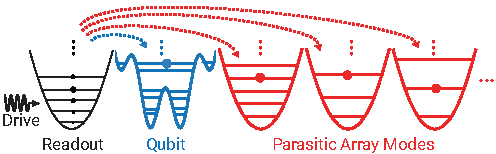
\includegraphics[width=\linewidth]{Figures/Demo.pdf}
    \caption{{\bf Schematic of a PMIST process.} A parasitic effect where energy in a coherent state of the driven readout mode (black) excites extraneous linear modes (red) and the nonlinear qubit mode (blue) simultaneously. 
    }
    \label{fig:demo}
\end{figure}
%%%%%%%%%%%%%%%%%%%%%%%%%%%%%%%%%%%%%

Similar detrimental transitions need examination for fluxonium to find ways to suppress such effects. The fluxonium circuit is fundamentally different and needs independent analysis. For example, the enhanced nonlinearity can dramatically change the number and likelihood of potential transitions~\cite{nesterov2024measurement,xiao2023diagrammatic}. In this article, we provide a comprehensive analysis of a unique MIST mechanism in fluxonium that arises due to the internal modes of the JJA during fluxonium readout (see Fig.~\ref{fig:demo}). We show that for realistic parameters and drive powers, deleterious resonant processes that simultaneously excite the qubit and an internal mode can occur. We term these processes parasitic MIST or PMIST. This can be viewed as an example of a more general problem: how is the physics of MIST modified in the presence of a structured environment?

We focus on a heavy fluxonium qubit operated at its flux sweet spot (cf~Fig.~\ref{fig:meas_circuit}) and investigate MIST, considering the coupling to the most relevant JJA internal modes. We treat the readout as an effective classical drive on the fluxonium-plus-JJA system and use an adiabatic Floquet branch analysis to identify dominant MIST processes. This method was used for transmon studies in Refs.~\cite{cohen2023reminiscence,dumas2024unified}. We also validate this approach through full time-dependent simulations.  
Our work goes beyond showing that such processes could be relevant. We discuss how they provide a mechanism for degrading qubit coherence even after measurements are complete (via dephasing from dispersive couplings to the excited internal modes). We also discuss how alternate circuit designs affect PMIST processes, focusing on how modifications affect the parasitic mode to qubit coupling strengths. Our analysis suggests that in optimizing fluxonium readout, parasitic JJA modes introduce additional constraints on the circuit design. We stress that our analysis is not an exhaustive study of MIST effects in fluxonium readout but aims to show how new mechanisms involving internal JJA degrees of freedom arise in realistic setups.

%%%%%structure%%%%%%
The remainder of this article is structured as follows. Sec.~\ref{sec:Fluxonium} analyzes the full circuit, including fluxonium, JJA, and readout resonator. Using a standard harmonic approximation~\cite{viola2015collective}, we derive qubit-parasitic mode coupling strengths and lower-bound parasitic mode effects during readout. Sec.~\ref{sec:MIST} analyzes readout dynamics, including MIST processes and dephasing from parasitic modes. Sec.~\ref{sec:expressions} examines the effects of varying coupling strengths between the qubit and a JJA internal mode on PMIST and investigates different ranges of readout frequencies and parasitic mode frequencies using an energy-conservation picture. In the concluding Sec.~\ref{sec:conclusion}, we discuss directions for future work.

%%%%%%%%%%%%%%%%%%%%%%%%%%%%%%%%%
\begin{figure}[t]
\centering    
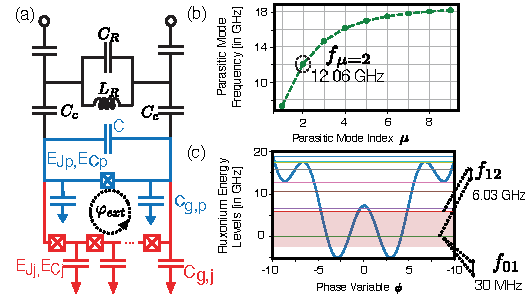
\includegraphics[width=\linewidth]{Figures/Meas_Circuit.pdf}
\caption{{\bf Fluxonium readout circuit, qubit, and array modes' spectrum.} (a) The color scheme shows primary components that correspond to various modes, shown in Fig.~\ref{fig:demo} when a JJA fluxonium circuit is connected to a readout resonator (R). The subscripts $p,j$ denote components of the phase-slip junction and the JJA, respectively. This circuit shows coupling capacitances ($C_\textrm{c}$), readout frequency parameters ($\omega_\textrm{r}=1/\sqrt{L_\textrm{R}C_\textrm{R}}$), parasitic ground capacitances in JJA ($C_\textrm{g,j}$) and next to the phase-slip junction ($C_\textrm{g,p}$). The differential capacitance $C$ adjusts the charging energy of the qubit mode (see Table~\ref{tab:readout_params}). (b) Fluxonium mode energy levels in units of $h$, with the highlighted area showing the first three levels essential for certain readout schemes~\cite{zhang_universal_2021}. (c) Parasitic mode frequencies $\omega_\mu/2\pi$. The lowest even mode $\mu = 2$ has the strongest coupling to the qubit (see Fig.~\ref{fig:coupling-strength}).
}
\label{fig:meas_circuit}
\end{figure}
%%%%%%%%%%%%%%%%%%%%%%%%%%%%%%%%%

%%%%%%%%%%%%%%%%%%%%%%%%%%%%%%%%%
\renewcommand{\arraystretch}{1.5} % Adjust the value as needed
\begin{table}[htb]
\centering
\begin{tabular}{|c|c|c|c|c|c|c|c|c|c|}
    \hline
     $N$ & $\varphi_{\textrm{ext}}$ & $E_{\textrm{J}_\textrm{p}}$ & $E_{\textrm{C}_\textrm{p}}$ & $E_{\textrm{C}}$ & $E_{\textrm{C}_\textrm{j}}$ & $E_{\textrm{J}_\textrm{j}}$ & $E_{C_\textrm{g,j}}$ & $E_{C_\textrm{g,p}}$ & $E_{\textrm{c}}$ \\
    \hline
    $122$ & $0.5\Phi_0$ & $7.30$ & $1.46$ & $17$ & $0.74$ & $60$ & $194$ & $1.94$ & $19.40$ \\
    \hline
\end{tabular}
\caption{{\bf Circuit parameters for Fig.~\ref{fig:meas_circuit}(a) inspired by Ref.~\cite{zhang_universal_2021}.} All energies are given in GHz. Here $\Phi_0=h/2e$ denotes the magnetic flux quantum. The capacitive energies $E_{\textrm{C}'}=\frac{19.4}{{C'}(\mathrm{fF})} \ \mathrm{GHz}$ are computed from the corresponding capacitances $C'$. See Table~\ref{tab:params} in App.~\ref{app:Hamiltonian} for the values of capacitances.}
\label{tab:circuit_params}
\end{table}
%%%%%%%%%%%%%%%%%%%%%%%%%%%%%%%%%



%%%%%%%%Our techniques and observations%%%%%%%%%%%%%




\renewcommand{\arraystretch}{1.5} % Adjust the value as needed

%%%%%%%%%%%%%%%%%%
\begin{table*}[tb]
    \centering
\begin{tabular}{|c|c|c|c|c|c|c|c|c|c|c|c|c|}
    \hline
    \textbf{Qubit ($\phi$) $\&$}&$\omega_{01}/2\pi$&$\omega_{12}/2\pi$ &$\tilde{E}^\phi_\textrm{c}$ &$g_{\phi \textrm{r}}/2\pi$&$\chi_{\phi \textrm{r}}(01)/2\pi$&$\chi_{\phi \textrm{r}}(12)/2\pi$&$\omega_\textrm{r}/2\pi$&$\kappa_\textrm{r}/2\pi$\\
    \cline{2-9}
\textbf{Readout ($r$)}&$30 \ \mathrm{MHz}$& $6.04 \ \mathrm{GHz}$ & $0.92 \ \mathrm{GHz}$& $25.50 \ \mathrm{MHz}$& $0.18 \ \mathrm{MHz}$&$0.98 \ \mathrm{MHz}$&$8.50 \ \mathrm{GHz}$&$1 \ \mathrm{MHz}$\\    
\hline\textbf{Parasitic-Mode} & \multicolumn{2}{c|}{} & $g_{\phi\mu}/2\pi$&$g_{\mu \textrm{r}}/2\pi$&$\chi_{\phi\mu}(01)/2\pi$&$\chi_{\phi\mu}(12)/2\pi$&$\omega_\mu/2\pi$&$Q_\mu$\\
    \cline{4-9}
\textbf{($\mu=2$)}&\multicolumn{2}{c|}{} &$157 \ \mathrm{MHz}$& $4.22 \ \mathrm{MHz}$& $-1.10 \ \mathrm{MHz}$& $5 \ \mathrm{MHz}$& $12.06 \ \mathrm{GHz}$&$10^{4}$\\    
\hline
\end{tabular}
\caption{{\bf Measurement parameters for qubit mode $\phi$, readout mode $r$, and closest even parasitic mode $\mu=2$.} All quantities are derived and computed analytically using circuit parameters listed in Table~\ref{tab:circuit_params} (see Apps.~\ref{app:alt_circuits}-\ref{app:Hamiltonian} for details). \textbf{Qubit-Readout Parameters:} ($\omega_{ij}$) qubit $i\rightarrow j$ splitting frequency between fluxonium excited states $i, j$; ($\tilde{E}^\phi_\textrm{c}$) qubit charging energy; ($g_{\phi \textrm{r}}$) qubit-readout coupling; ($\chi_{\phi \textrm{r}}(ij)$) dispersive shift due to readout mode in the two-level $ij$ system; ($\omega_\textrm{r}$) readout mode frequency; ($\kappa_\textrm{r}$) decay rate of the readout resonator. \textbf{Parasitic-Mode Parameters:} ($g_{\phi \mu}$) qubit-parasitic coupling; ($g_{\mu \textrm{r}}$) parasitic-readout coupling; ($\chi_{\phi \mu}(ij)$) dispersive shift due to parasitic mode $\mu$ in the two-level $ij$ system; ($\omega_\mu$) mode frequency; and ($Q_\mu$) internal quality factor inspired by~\cite{masluk_microwave_2012}.}   \label{tab:readout_params}
\end{table*}
%%%%%%%%%%%%%%%%%%



%%%%%%%%%%%%%%%%%%%%%%%%%%%%%%%%%%%%%%%%%%%%%%%%%%%%%%%%%%%%%%%%%
%%%%%%%%%%%%%%%%%%%%%%%%%%%%%%%%%%%%%%%%%%%%%%%%%%%%%%%%%%%%%%%%%
%%%%%%%%%%%%%%%%%%%%%%%%%%%%%%%%%%%%%%%%%%%%%%%%%%%%%%%%%%%%%%%%%

\section{Fluxonium Readout Circuit}\label{sec:Fluxonium}


%%%%Fluxonium circuit%%%%%%%%%%%%%%%%%%%%%%
We consider a JJA-fluxonium circuit dispersively coupled to a readout mode as shown in Fig.~\ref{fig:meas_circuit}. We choose circuit parameters (as listed in Table~\ref{tab:circuit_params}) motivated by recent experiments on heavy fluxonium~\cite{zhang_tunable_2024,zhang_universal_2021, ding_high-fidelity_2023}. We also restrict attention to the flux ``sweet spot" that maximizes qubit coherence. This choice is expected to reduce the number of allowed transitions in the circuit, as transitions between parity-conserving states via first-order processes are forbidden in this case. For our parameters, the qubit frequency ($\omega_{01}/2\pi$) is $\sim 30 \ \mathrm{MHz}$ and the plasmon frequency (i.e., splitting frequency between first and second qubit excited states $\omega_{12}/2\pi$) is $\sim 6 \ \mathrm{GHz}$ (see Table~\ref{tab:readout_params} for a full list of readout parameters).
 

%%%%%%%%%JJA+assumptions%%%%%%%%%%%%%%%%
Our work specifically investigates the role of the JJA, which comprises the inductive shunt of the fluxonium. The array comprises $N$ junctions and $N-1$ ground capacitances ($C_{\textrm{g}_n}$)~\cite{manucharyan2009fluxonium}. We neglect disorder effects and take junction parameters and parasitic ground capacitances to be uniform in the array (i.e., $C_{\textrm{g}_1}=..=C_{\textrm{g}_\textrm{N}}$). This capacitance value is given by $C_\textrm{g,j}$, where the subscript $j$ indicates the parasitic ground capacitance in the JJA~\footnote{Note that the ground capacitances $C_{\textrm{g}_n}$ are distinct from the self-capacitance $\frac{19.4}{E_{C,j}(\mathrm{GHz})}\mathrm{fF}$ (see Table~\ref{tab:params}) across the junctions in the array, which set the junction array plasmon frequency \cite{catelani2011relaxation}}. As shown in Fig.~\ref{fig:meas_circuit}(a), two additional identical ground capacitances $C_{\textrm{g}_0}, C_{\textrm{g}_\textrm{N}}$ near the phase-slip junctions in blue (see Fig.~\ref{fig:meas_circuit}) may have different values compared to those in the interior of the array, i.e., $C_{\textrm{g}_0}=C_{\textrm{g}_\textrm{N}}\equiv C_\textrm{g,p}\neq C_\textrm{g,j}$. Note that the subscript $p$ indicates the parasitic ground capacitances next to the phase-slip junction.


The JJA fluxonium circuit has $N$ internal degrees of freedom~\cite{ferguson2013symmetries,viola2015collective}: one qubit mode ($\phi$) and $N-1$ internal modes ($\mu=1,2,...,N-1$). These internal modes are coupled via the ground capacitances and are referred to as the ``parasitic" modes of the JJA. 

In our notation, we label the readout mode as $r$. The charge and flux quadratures of the qubit mode are denoted by $\hat N_\phi$ and $\hat \phi$ where $[\hat \phi,\hat N_\phi]=i\hbar$. 

We simplify the problem by treating all but the qubit mode as harmonic oscillators; this is a good approximation for standard device parameters~\cite{ferguson2013symmetries,viola2015collective,dumas2024unified}. We denote the photon loss and gain operators of the linear modes $r,\mu$ using $\hat a_\textrm{r},\hat a_\mu$ and $\hat a_\textrm{r}^\dagger,\hat a_\mu^\dagger$, respectively. 

Setting $\hbar=1$, the Hamiltonian of our fluxonium circuit has the form~\cite{viola2015collective}

\begin{equation}
   \hat H =\hat{H}_\phi + \hat{H}_\mu + \hat{H}_\textrm{r} + \hat{H}_{\textrm{int}},\label{Hamiltonian_total}
\end{equation}
where the qubit Hamiltonian $\hat{H}_\phi$ (with JJA inductive energy $E_\textrm{L}=E_{\textrm{J}_\textrm{j}}/N$) is 
\begin{equation}
\hat{H}_\phi / 2\pi = 4\tilde{E}^\phi_\textrm{c} \hat N_\phi^2+ E_{\textrm{J}_\textrm{p}}\cos{\hat\phi}+E_\textrm{L}\hat \phi^2 /2,\label{eq:Hphi}
\end{equation}
the junction array and readout Hamiltonians are $\hat{H}_\mu = \sum_{\mu}\omega_\mu \hat a_\mu^\dagger \hat a_\mu$ and $\hat{H}_\textrm{r} = \omega_\textrm{r} \hat a_\textrm{r}^\dagger \hat a_\textrm{r}$, respectively. The qubit charging energy
$\tilde{E}^\phi_\textrm{c}$ (see Table~\ref{tab:readout_params}) deviates from the target value of $E_{\textrm{c}}^{\phi}=1 \ \mathrm{GHz}$ due to parasitic capacitance. The coupling between the three modes is described by the interaction Hamiltonian
\begin{align}\label{eq:int_hamiltonian}
\hat{H}_{\textrm{int}} &= -i\sum_{\mu} g_{\phi\mu} \frac{\hat N_\phi}{{N_{\phi,\mathrm{ZPF}}}} (\hat a_\mu-\hat a_\mu^\dagger)\nonumber \\ &\quad-ig_{\phi \textrm{r}} \frac{\hat N_\phi}{{N_{\phi,\mathrm{ZPF}}}} (\hat a_\textrm{r}-\hat a_\textrm{r}^\dagger) \nonumber \\&\quad+ \sum_{\mu} g_{\mu \textrm{r}} (\hat a_\textrm{r}-\hat a_\textrm{r}^\dagger)(\hat a_\mu-\hat a_\mu^\dagger).
\end{align}
For our parameters, the zero-point fluctuations of qubit charge are $N_{\phi,\mathrm{ZPF}}=0.36$. Values for all remaining parameters are given in Table~\ref{tab:readout_params}. Explicit expressions for the $g_{\phi\mu}$ are discussed in Sec.~\ref{sec:expressions}.
 
%%%%%choosing the lowest even mode %%%%%
We find that the lowest-frequency even parasitic mode $\mu=2$ has the strongest coupling to the qubit mode (see Fig.~\ref{fig:coupling-strength} in App.~\ref{app:coupling}); corresponding parameters are listed in Table~\ref{tab:readout_params}. The symmetry of the circuit in Fig.~\ref{fig:meas_circuit}(a) prevents coupling between all odd parasitic modes (including $\mu=1$) and other circuit modes~\cite{viola2015collective}. We derive the Lagrangian of the symmetric circuit to prove this result, for completeness, in App.~\ref{app:alt_circuits}. In addition, we derive the Lagrangian for an asymmetric circuit with a different grounding configuration, inspired by~\cite{zhang_universal_2021}. We show that this asymmetric circuit couples the lowest frequency parasitic mode $\mu=1$ and is more detrimental for PMIST. Moreover, Fig.~\ref{fig:coupling-strength} shows that the $\mu=2,4,6$ parasitic modes couple to the qubit with a strength $g_{\phi\mu}$ that is stronger than the qubit-readout coupling $g_{\phi \textrm{r}}$.

Given these insights, in the rest of this work we focus on the symmetric circuit from Fig.~\ref{fig:meas_circuit} using parameters given by Tables~\ref{tab:circuit_params}-\ref{tab:readout_params} in Eq.~\ref{Hamiltonian_total}. Further, our description retains only the strongest coupled parasitic mode $\mu = 2$, along with the qubit and readout resonator. For details on other parasitic modes and their parameters, see App.~\ref{app:coupling}. Note that for our chosen parameters (see Table~\ref{tab:circuit_params}), the qubit couples roughly six times more strongly to the parasitic mode at $\mu=2$ than it does to the readout $r$~\footnote{In fact, the first four even parasitic modes have coupling strengths within a factor of $10$ of $g_{\phi \textrm{r}}$. See Fig.~\ref{fig:coupling-strength} in App.~\ref{app:coupling}}. We show that this strong coupling implies that the parasitic mode can play a significant role in measurement-induced state transitions, i.e., the PMIST effect that is the subject of this work.

\section{Parasitic-mode-Induced State Transitions: PMIST}\label{sec:MIST}

In this section, we analyze how the presence of a parasitic mode ($\mu=2$) affects the dynamics of a driven fluxonium circuit during a readout pulse. To simulate the linear drive on the readout resonator, we add a drive term $\hat{V}_\textrm{d}=i\xi (\hat a_\textrm{r}-\hat a_\textrm{r}^\dagger)\cos{\omega_\textrm{d} t}$ to the system Hamiltonian in Eq.~\ref{Hamiltonian_total}. Considering the fluxonium qubit mode, parasitic modes, and readout resonator, a full numerical analysis of several excitations in the circuit would require a prohibitively large Hilbert space. To truncate our Hilbert space to feasible dimensions for numerical simulations, we include only a single parasitic mode $\mu=2$ (as previously justified in Sec.~\ref{sec:Fluxonium}) and replace the readout mode with a classical drive term~\cite{cohen2023reminiscence,dumas2024unified,xiao2023diagrammatic} (see derivation in App.~\ref{app:semi-classical}). Under this semi-classical approximation, the driven circuit Hamiltonian includes the qubit mode $\phi$ and the parasitic mode at $\mu=2$, and is
\begin{align}
  \hat H_\textrm{s.c.}(\bar n_\textrm{r})=\hat H_0+\hat V_\textrm{s.c.}(\bar n_\textrm{r}).  \label{eq:drive_Ham}
\end{align}
Here, the bare Hamiltonian is
\begin{align}
\hat H_0=\hat H_\phi+\hat H_{\mu}+\frac{g_{\phi\mu}\hat N_\phi \hat N_\mu }{N_{\phi,\mathrm{ZPF}}N_{\mu,\mathrm{ZPF}}} \label{eq:bare_ham} 
\end{align}
and the modified drive term $V_\textrm{s.c.}$ is
\begin{align}
    \hat V_\textrm{s.c.}(\bar n_\textrm{r})&=\frac{\xi_{\phi \textrm{r}}(\bar n_\textrm{r})}{N_{\phi,\mathrm{ZPF}}} \hat N_\phi\cos{\omega_\textrm{d} t}+\frac{\xi_{\mu \textrm{r}}}{N_{\mu, \mathrm{ZPF}}}(\bar n_\textrm{r}) \hat N_\mu\cos{\omega_\textrm{d} t}\label{eq:drive},
\end{align}
where the effective drive amplitudes $\xi_{\mu(\phi) r}(\bar n_\textrm{r})=2g_{\mu(\phi) r}\sqrt{\bar n_\textrm{r}}$, and $\bar n_\textrm{r}$ denotes the average number of photons in the readout cavity. In the remaining text, we refer to the quantities $\xi_{\phi \textrm{r}/\mu \textrm{r}}$ as ``qubit drive strengths" and ``parasitic drive strengths", respectively.

Our primary focus is to analyze PMIST processes that introduce simultaneous transitions in the parasitic mode and the qubit mode. To identify the likely state transitions in the driven circuit, we first examine the energy eigenstates of the bare Hamiltonian $\hat{H}_0$ in Eq.~\ref{eq:bare_ham}. These states are hybridized fluxonium-parasitic mode states, and we label them as $\ket{\tilde{k}, \tilde{n}}$. A given state $\ket{\tilde{k}, \tilde{n}}$ corresponds to the eigenstate that has the maximum overlap with ``bare" fluxonium and parasitic mode states $\ket{k}_\phi\otimes\ket{n}_\mu$, i.e., the eigenstates of $H_{\phi}$ and $H_{\mu}$.

In what follows, we identify relevant state transitions in the driven fluxonium plus parasitic mode system. First, we perform an analysis based on the Floquet eigenstates of our system at a given fixed drive power~\cite{khezri2023measurement,cohen2023reminiscence,dumas2024unified}. We then simulate the drive ring-up to some chosen final photon number $\bar{n}_\textrm{r}$ and identify potential state transitions. We do this for a range of drive frequencies $\omega_\textrm{d}$. We find that the presence of the parasitic mode $\mu=2$ significantly increases the number of MIST processes in the system. We analyze the processes that cause these transitions and quantify their rates using perturbative approaches and Landau Zener probability calculations~\cite{ikeda2022floquet}. We also show that the residual population in the parasitic modes, after a readout pulse, can lead to significant dephasing of the reset qubit mode, limiting the performance of the qubit for future use.

%%%%%%%%%%%%%%%%%%%%%%%%%%%%%%%%%%
\subsection{Floquet branch analysis method} 

%%%%%%%%%%%%%%%%%%%%%%%%%%%%%%%%%%
\begin{figure}[!htb]
    \centering
    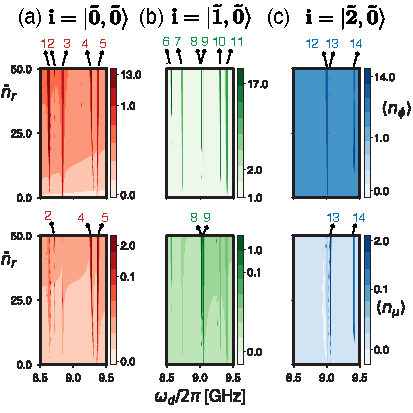
\includegraphics[width=0.5\textwidth]{Figures/Floquet_min.pdf}
    \caption{{\bf MIST and PMIST processes as seen in Floquet branch simulations.}  
    Each column corresponds to the branch associated with a specific undriven (but dressed) eigenstate $i=\ket{\tilde{k},\tilde{0}}$.  
    \textbf{Top row:} Average fluxonium excitation number in the given branch $\langle n_\phi\rangle$, as a function of drive power ($\propto\bar{n}_\textrm{r}$) and drive frequency $\omega_\textrm{d}$. \textbf{Bottom row:} Average excitation number of the $\mu=2$ parasitic mode, $\langle n_\mu\rangle$. Color scales use a log scaling to help visualize all transitions. Arrows and numbers indicate each transition (with numbers corresponding to Table~\ref{tab:PMIST}). See Figs.~\ref{fig:Trans0}-\ref{fig:Trans2} of App.~\ref{app:Floquet-trans} for corresponding behavior of quasienergies.}
    \label{fig:Floquet}
\end{figure}
\begin{table*}[t]
    \centering
    \begin{tabular}{w{c}{2.0cm}w{c}{3.0cm}w{c}{2.0cm}w{c}{2.0cm}w{c}{2.5cm}w{c}{1.5cm}w{c}{2.5cm}}
\hline
\shortstack{\\\textbf{Transition }\\\textbf{No.}\\\textbf{ (see Fig.~\ref{fig:Floquet})}} &\shortstack{\\\textbf{Fluxonium}\\\textbf{MIST}\\\textbf{Process}} &\shortstack{\\\textbf{Threshold}\\\textbf{Drive}\\\textbf{Photon ($\bar n_\textrm{r}$)}}& \shortstack{\\\textbf{Drive}\\\textbf{Frequency}\\($\omega_\textrm{d}/2\pi$)}& \shortstack{\\\textbf{Quasienergy}\\\textbf{Gap}\\($\Delta_\textrm{ac}$)}& \textbf{PMIST}&\shortstack{\textbf{Drive Photons}\\\textbf{Absorbed}\\\textbf{(see Fig.~\ref{fig:trans_prof})}}\\
\hline
\rule{0pt}{4ex}$1.$&$\color{BrickRed}{\ket{\tilde{0},\tilde{0}}}$$\xleftrightarrow []{\hspace{1em}}\ket{\tilde{13},\tilde{0}}$&$13$ &$8.64 \ \mathrm{GHz}$&$0.90 \ \mathrm{MHz}$&$\times$ & $3$\\
%\hline
$2.$&$\color{BrickRed}{\ket{\tilde{0},\tilde{0}}}$$\xleftrightarrow[]{\hspace{1em}}\ket{\tilde{4},\tilde{2}}^*$ &$48$&$8.71 \ \mathrm{GHz}$&$0.06 \ \mathrm{MHz}$&$\color{BrickRed}{\checkmark}$ & $4$\\
%\hline
$3.$&$\color{BrickRed}{\ket{\tilde{0},\tilde{0}}}$$\xleftrightarrow[]{\hspace{1em}}\ket{\tilde{8},\tilde{0}}$ &$\sim 0$&$8.84 \ \mathrm{GHz}$&$-$&$\times$ &$2$\\
%\hline
$4.$&$\color{BrickRed}{\ket{\tilde{0},\tilde{0}}}$$\xleftrightarrow[]{\hspace{1em}}\ket{\tilde{6},\tilde{1}}^*$&$46$&$9.25 \ \mathrm{GHz}$&$1.63 \ \mathrm{MHz}$&$\color{BrickRed}{\checkmark}$ &$2$\\
$5.$&$\color{BrickRed}{\ket{\tilde{0},\tilde{0}}}$$\xleftrightarrow[]{\hspace{1em}}\ket{\tilde{3},\tilde{1}}$ &$12$&$9.36 \ \mathrm{GHz}$&$0.56 \ \mathrm{MHz}$&$\color{BrickRed}{\checkmark}$ &$2$\\
%\hline
$6.$&$\color{ForestGreen}{\ket{\tilde{1},\tilde{0}}}$$\xleftrightarrow[]{\hspace{1em}}\ket{\tilde{17},\tilde{0}}$ &$32$&$8.56 \ \mathrm{GHz}$&$0.25 \ \mathrm{MHz}$&$\times$ & $4$\\
%\hline
$7.$&$\color{ForestGreen}{\ket{\tilde{1},\tilde{0}}}$$\xleftrightarrow[]{\hspace{1em}}\ket{\tilde{7},\tilde{0}}$ &$4$&$8.73 \ \mathrm{GHz}$&$0.74 \ \mathrm{MHz}$&$\times$ & $2$\\
%\hline
$8.$&$\color{ForestGreen}{\ket{\tilde{1},\tilde{0}}}$$\xleftrightarrow[]{\hspace{1em}}\ket{\tilde{12},\tilde{1}}$&$19$&$9.02 \ \mathrm{GHz}$&$0.12 \ \mathrm{MHz}$&$\color{ForestGreen}{\checkmark}$ & $4$\\
%\hline
$9.$&$\color{ForestGreen}{\ket{\tilde{1},\tilde{0}}}$$\xleftrightarrow[]{\hspace{1em}}\ket{\tilde{2},\tilde{1}}$  &$11$&$9.05 \ \mathrm{GHz}$&$0.66 \ \mathrm{MHz}$&$\color{ForestGreen}{\checkmark}$ & $2$\\
%\hline
$10.$&$\color{ForestGreen}{\ket{\tilde{1},\tilde{0}}}$$\xleftrightarrow[]{\hspace{1em}}\ket{\tilde{14},\tilde{0}}$ &$7$&$9.31 \ \mathrm{GHz}$&$0.50 \ \mathrm{MHz}$&$\times$ & $3$\\
%\hline
$11.$&$\color{ForestGreen}{\ket{\tilde{1},\tilde{0}}}$$\xleftrightarrow[]{\hspace{1em}}\ket{\tilde{9},\tilde{0}}$ &$2$&$9.41 \ \mathrm{GHz}$&$1.19 \ \mathrm{MHz}$&$\times$ &$2$\\
%\hline
$12.$&$\color{RoyalBlue}{\ket{\tilde{2},\tilde{0}}}$$\xleftrightarrow[]{\hspace{1em}} \ket{\tilde{12},\tilde{0}}$ &$3$&$9.00 \ \mathrm{GHz}$&$0.73 \ \mathrm{MHz}$&$\times$ & $2$\\
%\hline
$13.$&$\color{RoyalBlue}{\ket{\tilde{2},\tilde{0}}}$$\xleftrightarrow[]{\hspace{1em}}\ket{\tilde{0},\tilde{2}}$&$38$&$9.06 \ \mathrm{GHz}$&$0.53 \ \mathrm{MHz}$&$\color{RoyalBlue}{\checkmark}$ & $2$\\
%\hline
$14.$&$\color{RoyalBlue}{\ket{\tilde{2},\tilde{0}}}$$\xleftrightarrow[]{\hspace{1em}}\ket{\tilde{5},\tilde{1}}^*$ &$49$&$9.41 \ \mathrm{GHz}$&$2.71 \ \mathrm{MHz}$&$\color{RoyalBlue}{\checkmark}$ & $2$\\
\hline
\end{tabular}
\caption{{\bf Measurement-induced-state-transition (MIST) observed in Fig.~\ref{fig:Floquet}.} Column $1$ lists the numbering used to mark the transitions in Fig.~\ref{fig:Floquet}. Here $\ket{\tilde{i},\tilde{j}}$ indicates the hybridized eigenstate of $H_0$ (see Eq.~\ref{eq:bare_ham}) which has the maximum overlap with the state $\ket{i}_\phi\otimes \ket{j}_{\mu=2}$ in the disjoint Hilbert space of qubit mode ($\phi$) and parasitic mode ($\mu=2$). Column $2$ lists the MIST processes that start  at the lowest average readout photon number $\bar n_\textrm{r}$ given by column $3$. In some cases, we use $\bar n_\textrm{r}\sim 0$ to indicate that the drive frequency is exactly resonant with the transition frequency between the two levels. A `$^*$'-marked state indicates hybridization at lower $\bar n_\textrm{r}$ due to preceding transitions~\footnote{$\ket{\tilde{4},\tilde{2}}^*:\ket{\tilde{4},\tilde{2}}\xleftrightarrow[]{\hspace{1em}}\ket{\tilde{14},\tilde{2}}$ at $\bar n_\textrm{r}=5, \omega_\textrm{d}/2\pi=8.71 \ \mathrm{GHz}$ with $\Delta_\textrm{ac}=4.0 \ \mathrm{MHz}$ absorbs $2$ drive photons\\$\ket{\tilde{6},\tilde{1}}^*:\ket{\tilde{6},\tilde{1}}\xleftrightarrow[]{\hspace{1em}}\ket{\tilde{3},\tilde{1}}$ at $\bar n_\textrm{r}\sim 0, \omega_\textrm{d}/2\pi=9.25 \ \mathrm{GHz}$\\$\ket{\tilde{5},\tilde{1}}^*:\ket{\tilde{5},\tilde{1}}\xleftrightarrow[]{\hspace{1em}} \ket{\tilde{17},\tilde{0}}$ at $\bar n_\textrm{r}=14, \omega_\textrm{d}/2\pi=9.41 \ \mathrm{GHz}$ with $\Delta_\textrm{ac}=4.2 \ \mathrm{MHz}$ absorbs $1$ drive photon}. Column $4$ represents the drive frequency $\omega_\textrm{d}/2\pi$ at which these transitions occur. Column $5$ yields the quasienergy gap at the avoided crossing labeled as $\Delta_\textrm{ac}$. Column $6$ indicates if the process cannot occur without the parasitic mode, denoted as PMIST. The various colors for the checkmarks indicate that the PMIST event involves the state $\ket{\tilde{0},\tilde{0}}$ (red), $\ket{\tilde{1},\tilde{0}}$ (green) or $\ket{\tilde{2},\tilde{0}}$ (blue). Column $7$ indicates the number of drive photons ($\#$) involved in the energy-conserving process, illustrated in Fig.~\ref{fig:trans_prof}, which is responsible for these transitions.
}
    \label{tab:PMIST}
\end{table*}
%%%%%%%%%%%%%%%%%%%%%%%%%%%%%%%%%%
%%%%%%%%%%%%%%%%%%%%%%%%%%%%%%%%%%

Our first numerical analysis involves calculating the Floquet eigenstates of $H_\textrm{s.c.}$ (see Eq.~\ref{eq:drive_Ham}) for various fixed values of the drive powers, as controlled by the average photon number $\bar n_\textrm{r}$. We do this by retaining the lowest 20 levels in the qubit subspace $\phi$ and 5 levels in the parasitic mode $\mu=2$\footnote{We show that our results hold when simulated with 30 levels in the qubit mode and 10 levels in the parasitic mode}; the truncation for this analysis is discussed further in App.~\ref{app:numerics}. Our goal is to use these results to make predictions for a readout pulse involving a time-dependent drive power, identifying possible transitions starting from a dressed state $\ket{i} =\ket{\tilde{\phi}, \tilde{\mu}}$ where $\phi\in\{0,1,2\}$ and $\mu=0$ (i.e., the parasitic mode is initially empty). With $\omega_\mu/2\pi=12.06 \ \mathrm{GHz}$, the analysis in this section considers the regime of negative detuning where $\omega_{\mu=2}>\omega_\textrm{d}=\omega_\textrm{r} \gg \omega_\textrm{q}$, and can be replicated for any other parasitic mode $\mu \neq 2$. Note that we also analyze the effects of an alternative circuit with $\omega_{\mu=2}/2\pi\sim 16 \ \mathrm{GHz}$ and $\omega_{01}/2\pi\sim 300 \ \mathrm{MHz}$ in Sec.~\ref{sec:expressions}.

Inspired by~\cite{dumas2024unified,cohen2023reminiscence}, we extract PMIST processes by tracking the evolution of the Floquet eigenstates as we increase the parameter $\bar{n}_\textrm{r}$, a method known as \emph{branch analysis}. We do this for a series of discrete values of $\bar{n}_\textrm{r}$ chosen to be integers. The simulation begins in a chosen eigenstate $\ket{i}_0$ of the bare Hamiltonian $\hat{H}_0 \equiv \hat{H}_\textrm{s.c.}[\bar{n}=0]$ (see Eq.~\ref{eq:bare_ham}). Next, we compute the Floquet eigenstates $\ket{m_1}$ of the Hamiltonian $\hat{H}_\textrm{s.c.}[\bar{n}_\textrm{r}=1]$, corresponding to a single photon increase in the readout resonator. We then identify the Floquet eigenstate of this Hamiltonian $\ket{i}_{\bar n_\textrm{r}=1}$ that has maximum overlap with $\ket{i}_{\bar n_\textrm{r}=0}$. We repeat this process iteratively, increasing $\bar{n}_\textrm{r}$ by one each time:
\begin{align}
\ket{i_{\bar n_\textrm{r}=l}}:\max_{m}|\braket{i_{\bar n_\textrm{r}=l-1}|{m}_{\bar n_\textrm{r}=l}}|^2.\label{eq:track_Floquet}   
\end{align}
We thus obtain a set of states $\ket{i}_0,\ket{i}_1,\ket{i}_2,...$ that we refer to as a branch. At a heuristic level, this trajectory of states describes the adiabatic evolution of the system as the drive power increases. The drive power in this trajectory increases to emulate a single photon increase in the readout resonator, i.e., $\delta \bar n_\textrm{r}=1$. This corresponds to a constant increase in drive powers (see Eq.~\ref{eq:drive}) $\delta |\xi_{\mu (\phi),\textrm{r}}|^2=4g_{\mu (\phi),\textrm{r}}^2$. We make this choice to emulate the more quantum approach to branch analysis captured in Ref.~\cite{shillito2022dynamics,dumas2024unified}. The probability for this ring-up is studied further for one of the transitions in Sec.~\ref{sec:LZ}. We emphasize that our analysis shows the impact of PMIST transitions and does not focus on identifying \emph{all} transitions caused by the $N$ parasitic modes in the fluxonium circuit.


We make these choices to observe population changes in the fluxonium potential, i.e., state transitions, as we increase the drive powers. In Eq.~\ref{eq:track_Floquet}, the overlaps between Floquet eigenstates are all computed at a fixed time within each drive period (i.e., at times $t_l = 2 \pi l/ \omega_\textrm{d}$). We have verified that our method yields the same results as Ref.~\cite{dumas2024unified} (where a time-averaged overlap was used). Note that the slower or more adiabatic the ring-up of the drive, the more likely it is to observe a state transition. To avoid weak transitions, we increase the drive using discrete steps of $\delta \bar n_\textrm{r}=1$, which corresponds to a linear increase in the drive powers. This choice uses a drive strength increment size $\delta |\xi_{\phi (\mu),\textrm{r}}|= 2g_{\phi(\mu),\textrm{r}}$, different from the driven transmon analysis in Refs.~\cite{dumas2024unified} where $\delta |\xi_{\phi,\textrm{r}}|\sim \kappa_\textrm{r}$, the readout resonator's decay rate. Thus, our simulations can also be used to understand the impact of parasitic state transitions due to a linearly increasing drive on the fluxonium circuit.


For each state $\ket{i_{\bar n_\textrm{r}=k}}$ in a given branch, we compute:
\begin{enumerate}
    \item The expectation value of the fluxonium excitation-number operator $\hat n_\phi=\sum_k k\ket{k}_\phi\bra{k}_\phi$, where $\ket{k}_\phi$ is the $k^{th}$ {\it bare} fluxonium energy eigenstate,
    \item The expectation value of the parasitic-mode number operator $\hat n_\mu=\hat a_{\mu}^\dagger \hat a_{\mu}$ (for the single mode $\mu=2$ that we retain), and 
    \item The quasi-energy of the state $E_i \mod (\omega_\textrm{d}/2\pi)$.
\end{enumerate}
We can thus identify MIST and PMIST transitions by detecting sudden changes in the number of qubit or parasitic mode excitations as $\bar{n}_\textrm{r}$ increases, indicating an unwanted drive-induced hybridization of eigenstates.


\subsection{Branch analysis PMIST predictions}

Fig.~\ref{fig:Floquet} illustrates our main result, showing examples of PMIST drive-induced transitions for initial states that have maximum overlap with states $\ket{0}_\phi$, $\ket{1}_\phi$, and $\ket{2}_\phi$ in the fluxonium subspace and the ground state $\ket{0}_{\mu=2}$ in the parasitic subspace. For each branch, we use a color map to plot the average excitation number of the qubit mode $\langle n_\phi \rangle$ (top row) and the parasitic mode $\langle n_\mu \rangle$, range of readout drive frequencies (horizontal axes), and final readout cavity average photon numbers $ \bar n_\textrm{r}$ (vertical axes).

Note that both the drive powers, of the qubit $\xi_{\phi \textrm{r}}$ and of the parasitic mode $\xi_{\mu \textrm{r}}$, are exclusively dependent on $\bar n_\textrm{r}$. Thus, we will often interchangeably call $\bar n_\textrm{r}$ the drive power. Results are shown for driven frequencies $\omega_\textrm{d} / 2 \pi$ in the range $8.5 - 9.5 \ \mathrm{GHz}$~\footnote{a relatively high-frequency choice, to reduce thermal, photon shot-noise induced dephasing in the qubit compared to lower-frequency bands}; other regimes are discussed in Sec.~\ref{sec:expressions}. For one-dimensional slices of the results at fixed $\bar n_\textrm{r}$, along with the quasi-energies, see App.~\ref{app:Floquet-trans}.


Any streak or sharp change in color intensity represents a sudden and significant jump in the qubit or parasitic mode population, i.e., MIST or PMIST. The parasitic transitions or PMIST correspond to simultaneous jumps in the population of the modes $\phi$ (Figs.~\ref{fig:Floquet}, top row) and $\mu=2$ (Figs.~\ref{fig:Floquet}, bottom row), as $\bar{n}_\textrm{r}$ varies. At these points, an avoided crossing in the quasi-energies of the Floquet states confirms the hybridization of the two states involved in the population exchange (see Figs.~\ref{fig:Trans0}-\ref{fig:Trans2} in App.~\ref{app:Floquet-trans}). Additional resonances may occur at alternate drive frequencies not shown in Fig.~\ref{fig:Floquet}. Table~\ref{tab:PMIST} lists significant transitions observed in our Floquet simulations and associated processes that cause them, identified through a perturbative analysis (see App.~\ref{app:Floquet-trans}) and energy conservation (shown later in Fig.~\ref{fig:trans_prof}). We note that certain MIST processes, including PMIST, involve transitions at the flux sweet spot~\cite{zhu_circuit_2013} between parity-conserving states, due to virtual excitations via non-parity-conserving states.

The above results clearly show that coupling to the JJA parasitic modes enables new MIST processes beyond what would be predicted by a fluxonium-only simulation. Further, we find that coupling to parasitic modes can alter and even disrupt transitions that would be predicted by a fluxonium-only calculation. For example, consider transition $14$ in Table~\ref{tab:PMIST}. For this drive frequency, if one neglects the qubit-parasitic mode coupling, one finds a MIST transition between $\ket{\tilde{2},\tilde{0}} \leftrightarrow \ket{\tilde{17},\tilde{0}}$ via the absorption of three drive photons. Including the parasitic mode, the nature of this process changes. As drive power (i.e., $\bar{n}_\textrm{r}$) increases, one first finds a transition between the states $\ket{\tilde{5},\tilde{1}}\leftrightarrow \ket{\tilde{17},\tilde{0}}$ at a threshold drive photon number of $\bar n_\textrm{r}=14$. As the drive power further increases, one obtains a transition $\ket{\tilde{2},\tilde{0}}\leftrightarrow \ket{\tilde{5},\tilde{1}}$ at $\bar n_\textrm{r}=41$, enabled by the earlier hybridization of $\ket{\tilde{5},\tilde{1}}$ and $\ket{\tilde{17},\tilde{0}}$.

Another qualitatively new feature that arises due to the parasitic modes is the possibility of MIST-like transitions where the qubit loses excitations. For example, consider transition $12$ in Table \ref{tab:PMIST}. In this process, two drive photons are absorbed, the fluxonium state has a downward transition $\ket{2}_\phi\rightarrow\ket{0}_\phi$, and the net energy released is used to excite the parasitic mode $\ket{0}_\mu\rightarrow \ket{2}_\mu$. By simple energy conservation, such an effect is not possible without a parasitic mode. In fact, this transition can even modify the $T_1$ lifetime of the $0-2$ fluxonium subspace, and not just contribute to leakage like general MIST phenomena.

Our results also display branch bunchings (see Figs.~\ref{fig:Trans0}, sub-panels $(2)$ and $(4)$, in App.~\ref{app:Floquet-trans} for reference) instead of crossings in the negative detuning regime. This is contrary to Ref.~\cite{dumas2024unified} where such branch bunching has been observed only in the positive detuning $(\omega_\textrm{q}>\omega_\textrm{r})$ regime.  Consider for example transitions $3$ and $4$ in Table \ref{tab:PMIST}. Here, we are  driving at a frequency that exactly matches the transition frequency between two non-computational states, such that these states immediately start to hybridize into an equal superposition of the two 
original undriven states.  For example, in transition $4$, the readout drive frequency exactly matches the $\ket{3}_\phi \rightarrow \ket{6}_\phi$ transition frequency at zero readout excitations. In this case, levels $\ket{3}_\phi$ and $\ket{6}_\phi$ hybridize for any non-zero drive power $\bar n_\textrm{r}$  (see Fig.~\ref{fig:Trans0} in App.~\ref{app:Floquet-trans}). While this effect is not limited to PMIST, we highlight that the presence of parasitic modes can result into more exotic transitions transitions. For example, in transition  $4$, one such transition between the states $\ket{\tilde{3},\tilde{1}}$ and $\ket{\tilde{6},\tilde{1}}$, where the parasitic mode was excited, eventually lead to a PMIST effect involving the computational state $\ket{\tilde{0},\tilde{0}}$. See Fig.~\ref{fig:Trans0}, sub-panel ($4$), for explicit population and quasienergy plots involving the three states.


Our findings reveal that for our specific circuit choice, JJA parasitic modes can become significantly populated, as we show in Fig.~\ref{fig:Floquet}. Having identified key transitions that cause these effects, we now calculate the transition rates in detail and the consequences on qubit coherence.

 \begin{figure}[t]
    \centering
    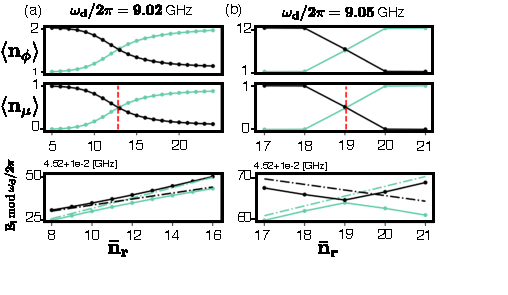
\includegraphics[width=\linewidth]{Figures/Floquet_011.pdf}
    \caption{{\bf PMIST processes including state $\ket{\tilde{1},\tilde{0}}$.} Examples of PMIST using transitions \textbf{(a)} $8$ and \textbf{(b)} $9$ from Table~\ref{tab:PMIST} involving the $\ket{\tilde{1},\tilde{0}}$ state, with maximum overlap to the un-hybridized state $\ket{1}_\phi\otimes\ket{0}_{\mu=2}$. \textbf{Top row:} Qubit mode average occupation $\braket{n_\phi}$. \textbf{Middle row:} Parasitic mode average occupation $\braket{n_\mu}$. \textbf{Bottom row:} $\tilde{E}_i=E_i \ \textrm{mod} \ \omega_\textrm{d}$ where $E_i$ is the Stark-shifted eigen-energy (dashed) obtained from first-order perturbative calculations, or quasi-energy (solid) obtained from Floquet simulations showing avoided crossings. Plots are extracted from numerical data used in Fig.~\ref{fig:Floquet}. The data points are connected by lines for visual aid.}
    \label{fig:011}
\end{figure}

For further insights, we now examine in more detail how the quasienergies and excitation numbers change as a function of drive power $\bar{n}_\textrm{r}$ when we pass through an avoided crossing associated with a PMIST process. Figs.~\ref{fig:011}(a,b) show explicitly how average qubit and parasitic mode excitation numbers change as a function of drive power $f(\bar n_\textrm{r})$ for fixed drive frequency corresponding to $8,9$ (respectively) in Table~\ref{tab:PMIST}. Both these transitions involve starting in the qubit's first excited state (i.e., branches associated with the undriven state $\ket{\tilde{1},\tilde{0}}$). The simultaneous exchange of population in the qubit mode $\phi$, shown in the top panels, and the parasitic mode $\mu=2$, shown in the middle panels, confirms that the transitions are indeed PMIST.

The bottom panel of Fig.~\ref{fig:011} shows the corresponding behavior of the branch quasi-energies as a function of drive power, for the same drive parameters. We plot both quasi-energies from the Floquet calculations and the predictions of a perturbative calculation including drive-induced Stark shifts (see App.~\ref{app:stark-shift} for details). For Fig.~\ref{fig:011}, the perturbative calculations predict the onset of an avoided crossing at a drive power close to the value derived from the Floquet simulations. Note that these transitions occur at relatively modest average readout cavity photon numbers $\bar n_\textrm{r}=11,19$.

\subsection{Transition probability}\label{sec:LZ}
\begin{figure}[t]
    \centering
    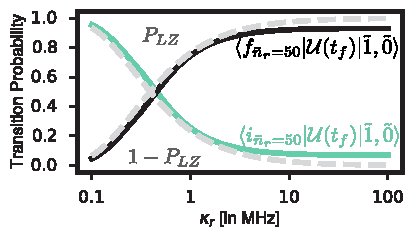
\includegraphics[width=\linewidth]{Figures/LZ.pdf}
    \caption{
        {\bf PMIST transition probabilities as a function of readout cavity ring-up rate.}
        We plot the probabilities for adiabatic (green) and diabatic (black) transitions for a time-dependent ring-up of the average cavity photon number from $\bar{n}_\textrm{r} = 0$ to $\bar{n}_\textrm{r} = 50$, for different choices of the cavity damping rate $\kappa_\textrm{r}$, which controls the speed of the sweep (see text). We start the system in the qubit's first excited state $\ket{\tilde{1},\tilde{0}}$. The drive frequency is $\omega_\textrm{d}/2\pi=9.05 \ \mathrm{GHz}$, corresponding to the crossing shown in Fig.~\ref{fig:011}(b). Here, $\ket{f_{\bar n_\textrm{r}=50}}$ and $\ket{i_{\bar n_\textrm{r}=50}}$ are the final states in the end of branch analyses for $\ket{\tilde{2},\tilde{1}}$ and $\ket{\tilde{1},\tilde{0}}$, respectively. The time-evolution operator is denoted by $\hat{\mathcal{U}}(t_\textrm{f})=\mathcal{T}\exp\big(-i\int^{t_\textrm{f}}_{0} \hat H_\textrm{s.c.}(t)dt\big)$, where $\mathcal{T}$ indicates time-ordering and $t_\textrm{f}=10/\kappa_\textrm{r}$. The adiabatic (green) curve corresponds to an unwanted PMIST transition. We also plot the predictions of the Floquet branch analysis combined with a Landau Zener approximation for the probabilities (gray), which are in excellent agreement over a wide range of $\kappa_\textrm{r}$.}
    \label{fig:LZ}
\end{figure}

Our Floquet branch analysis gives strong evidence that MIST and PMIST transitions will occur during the ring-up of the resonant during a readout pulse.  Here, we validate this approach by focusing on a specific transition, and we show (via explicit time-dependent simulations) that it occurs as predicted.  We also show that this full-time-domain simulation is in agreement with a Landau-Zener analysis that takes as inputs the result of the Floquet branch analysis.    

Our Floquet branch analysis gives strong evidence that MIST and PMIST transitions will occur during the ring-up of the resonator during a readout pulse. Here, we validate this approach by focusing on a specific transition and show (via explicit time-dependent simulations) that it occurs as predicted. We also show that this full-time-domain simulation is in agreement with a Landau-Zener analysis that takes as inputs the result of the Floquet branch analysis.

We focus on the PMIST transition shown in Fig.~\ref{fig:011}(b), which corresponds to an avoided crossing energy gap of $\Delta_\textrm{ac}=0.66$ MHz. We perform a full time-dependent simulation of $\hat H_\textrm{s.c.}$ in Eq.~\ref{eq:drive_Ham}, using time-dependent drive powers determined by the time-dependent average readout cavity photon number in the form:
\begin{align}
    \bar n_\textrm{r}(t)&=\bar n_\textrm{r}(1-e^{-\kappa_\textrm{r} t/2})^2.\label{eq:LZ-n}
\end{align}
This corresponds to the ring-up of a resonantly driven cavity with a damping rate $\kappa_\textrm{r}$~\cite{khezri2023measurement,dumas2024unified,cohen2023reminiscence}.

To calculate transition probabilities in this full-time-dependent simulation, we initiate the system in the dressed state $\ket{\tilde{1},\tilde{0}}$, evolve under $\hat{H}_\textrm{s.c.}(t)$ from $t=0$ to $t=10 / \kappa_\textrm{r}$, and then compute the overlap of this state with the Floquet branches of the two states $\ket{i}=\ket{\tilde{1},\tilde{0}}$ and $\ket{f}=\ket{\tilde{2},\tilde{1}}$ associated with our predicted transition. We then repeat this calculation for different choices of $\kappa_\textrm{r}$, examining how the transition probabilities vary, with the results shown in Fig.~\ref{fig:LZ}. As expected, the probability of remaining adiabatic (green curve) decreases as one increases $\kappa_\textrm{r}$. Note that at large $\kappa_\textrm{r}$, adiabatic evolution corresponds to a detrimental PMIST transition, as the most likely final state $\ket{\tilde{2}, \tilde{1}}$ has an extra qubit and parasitic mode excitation compared to the initial state $\ket{\tilde{1}, \tilde{0}}$.


For small $\kappa$, the above probabilities are in agreement with the predictions of our Floquet branch analysis combined with a Landau-Zener approximation to the probability of a non-adiabatic transition~\cite{ikeda2022floquet,dumas2024unified} (see App.~\ref{app:LZ}). These probabilities ($P_{\mathrm{LZ}}$) are shown in gray in Fig.~\ref{fig:LZ}. We see agreement for most of the values of $\kappa_\textrm{r}$ between the time-domain simulations and our Landau-Zener calculations using the Floquet quasi-energies. For large $\kappa_\textrm{r}$, we find that the probabilities do not saturate to $1$ and $0$ as would be expected in the standard Landau-Zener problem; they do, however, sum to unity (hence transitions to additional levels are not contributing). We attribute this small deviation to dressing effects that go beyond the simple two-level Landau-Zener paradigm.

\subsection{Post-readout qubit dephasing}\label{sec:dephasing}

The new PMIST processes we identify here can also potentially create errors \textit{after} the readout pulse is complete, as they lead to a new dephasing channel. A PMIST process results in a JJA parasitic mode having a residual excitation post-readout. As there is a non-zero dispersive coupling $\chi_{\mu \phi}$ between these modes and the qubit, and as these modes are believed to have relatively large internal quality factors $Q\sim 10^{4}$~\cite{masluk_microwave_2012, masluk2013reducing}, this will lead to the qubit acquiring a random phase (tied to the random time at which the parasitic mode relaxes). Below, we show master equation simulation results which quantify the scale of phase errors that would result from such processes.

\begin{figure}[htb]
    \centering
    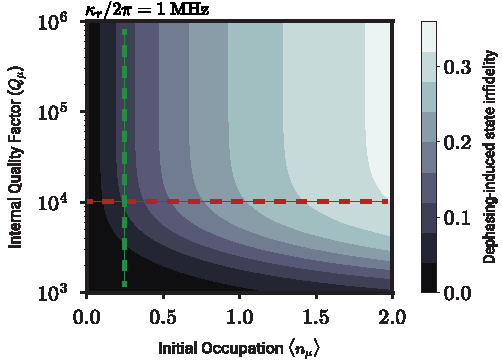
\includegraphics[width=\linewidth]{Figures/dephasing.pdf}
    \caption{{\bf Dephasing error probability due to random decay of an excited parasitic mode, after PMIST, various internal parasitic quality factors.} The horizontal red line shows the quality factor quoted in~\cite{masluk_microwave_2012}. The green line shows the dephasing error probability for transition $9$ for various quality factors at $\kappa_\textrm{r}/2\pi=1 \ \mathrm{MHz}$ (see Figs.~\ref{fig:011}(b) and~\ref{fig:LZ}).}
    \label{fig:dephasing}
\end{figure}

For concreteness, we consider a readout pulse with a frequency corresponding to the PMIST transition labeled $9$ in Fig.~\ref{fig:011}(b) and a cavity damping rate $\kappa_\textrm{r}/2\pi=1 \ \mathrm{MHz}$ (which determines the ring-up time of the cavity to the maximum drive powers given by $\bar n_\textrm{r}=50$). For these parameters, our previous simulations and Landau-Zener analysis suggest that at the end of the readout pulse, the parasitic mode will have an average non-zero excitation $\braket{n_\mu}=0.25$. In fact, for many transitions this population can be as high as $\braket{n_\mu}=2.0$ as shown in Table~\ref{tab:PMIST}. We now ask how the decay of such a population will dephase the fluxonium (assuming it is prepared after readout in the state $\ket{+}=\frac{\ket{0}_\phi+\ket{1}_\phi}{\sqrt{2}}$).

A master equation simulation illustrates the resulting qubit dephasing due to this mechanism.  We investigate a reduced system of the parasitic mode $\mu=2$ and the fluxonium qubit (modeled as a two level system), interacting under the dispersive Hamiltonian $\hat H_\theta/\hbar=\chi_{\phi\mu} \hat a_\mu^\dagger \hat a_\mu \sigma_\textrm{z}$, and with a loss dissipator having collapse operator $\sqrt{\kappa_\mu}\hat a_\mu$, describing the parasitic mode internal loss.  We start the system in a product state, where the parasitic mode has some initial non-zero occupation, and the qubit is in the pure state $\ket{+}$. 
We let the system evolve for a time $T_\textrm{f}=10/\kappa_\mu$ long enough to allow the parasitic mode to relax, and then compute the fidelity of the final qubit state with the initial state $\ket{+}$, defining the error probability be the corresponding infidelity.  
This quantity is plotted in Fig.~\ref{fig:dephasing}, both as a function of the initial parasitic mode occupancy $\braket{n_\mu}$ and its internal quality factor $Q_\mu$. \singh{We present an illustrative calculation where we initialize the parasitic mode in a thermal state with average occupation number equal to $n_\mu\in[0,2]$. Note that results quoted for dephasing in the text below do not change significantly if the parasitic mode was instead initialized a coherent state $\ket{\alpha}$ such that $|\alpha|^2=\braket{n_\mu}.$} We find that for an internal quality factor $Q_\mu$ of $10^{4}$, an initial population of $\braket{n_\mu}=0.25$ in the parasitic mode introduces a dephasing error probability $\epsilon \sim 0.1$, which is already past the threshold of the surface code~\cite{fowler2012surface}. The explicit time-dependent simulations shown in Fig.~\ref{fig:011} indicate that using a realistic readout power of $\sim 10$ photons, the final post-readout parasitic mode population is $\braket{n_\mu}\sim 0.25$.  This population would already be enough to lead to a significant post-readout dephasing effect. 


%%%%%%%%%%%%%%%
\section{Effects of Circuit Modifications on PMIST}\label{sec:expressions}
Let's explore how adjusting the qubit frequency, readout resonator frequency, and parasitic mode frequencies may affect unwanted transitions. We rely on derivations in Ref.~\cite{viola2015collective} for the circuit in Fig.~\ref{fig:meas_circuit} (see App.~\ref{app:alt_circuits} for the Lagrangian).


\subsection{Coupling strengths} \label{sec:coupling}

Fig.~\ref{fig:coupling-Floquet} identifies the main culprit behind PMIST as the fluxonium-parasitic-mode coupling, $g_{\phi \mu}$. We compare the results of Floquet branch analyses for the initial state $\ket{\tilde{1}, \tilde{0}}$ under different coupling conditions, drive frequencies, and amplitudes. Fig.~\ref{fig:coupling-Floquet}(a) reproduces as a reference the simulation results for our previous choice of coupling strengths $g_{\phi\mu}$ and $g_{\mu \textrm{r}}$. In contrast, Fig.~\ref{fig:coupling-Floquet}(b) shows the same simulation but with $g_{\phi \mu}$ set to zero. We observe that a non-negligible $g_{\phi\mu}$ is the main reason for PMIST effects. This is evident from the absence of parasitic transitions $(8,9)$ in the top panel, and no streak or sharp change in color indicating parasitic mode excitations in the bottom panel: for $g_{\phi \mu}=0$ the parasitic mode population always remains below $\braket{n_\mu}=10^{-4}$.

Further, Fig.~\ref{fig:coupling-Floquet}(c) shows that turning the parasitic-readout coupling to zero shows no reduction in PMIST. Thus, we can conclude that the qubit-readout coupling $g_{\phi \textrm{r}}$ alone does not cause significant transitions or PMIST processes without $g_{\phi \mu}$. Therefore, reducing the coupling strength $g_{\phi \mu}$ is a potential path to reducing the likelihood of PMIST processes.

\begin{figure}[t]
    \centering
    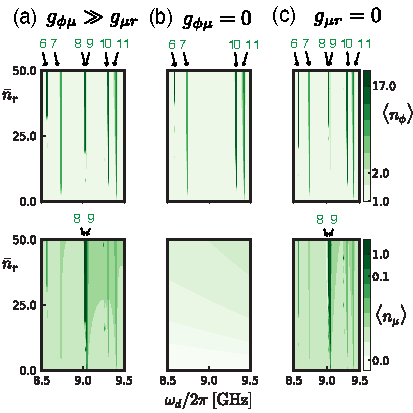
\includegraphics[width=\linewidth]{Figures/Floquet_coupling.pdf}
    \caption{
        {\bf Sensitivity of PMIST processes to parasitic mode coupling strengths.} Panels show the result of Floquet branch analyses for the circuit parameters in Table~\ref{tab:circuit_params}. MIST processes observed in Fig.~\ref{fig:Floquet} are labeled with numbers and indicated with arrows. \textbf{(a)} All parameters are the same as in Fig.~\ref{fig:Floquet}(b). \textbf{(b)} Same, except now we set the parasitic mode to qubit coupling $g_{\phi \mu}$ to zero. Note that all PMIST features are now gone. \textbf{(c)} Same as (a), but we now set the parasitic mode to readout resonator coupling $g_{\mu \textrm{r}}$ to zero. As with previous Floquet branch analysis plots, color scales use a log scale to make transitions more visible.}
    \label{fig:coupling-Floquet}
\end{figure}

Next, we analyze the dependence of these coupling strengths on circuit and readout parameters. As discussed, only even-index parasitic modes have a non-zero coupling to the qubit (see the Lagrangian in App.~\ref{app:alt_circuits}). The coupling strength $g_{\phi \mu}$ between an even parasitic mode and the qubit is given by
\begin{align}
\frac{g_{\phi\mu}}{2\pi}&=\frac{4}{\sqrt{2N}} \frac{\tilde{E}^\phi_\textrm{c}\tilde{E}^\textrm{e}_{\textrm{c},\mu}c_\mu}{E_{\textrm{g,j}}s_\mu^2} \cdot {N_\phi}_{\mathrm{ZPF}} \cdot {N_\mu}_{\mathrm{ZPF}},
\end{align}
where $c_\mu=\cos{\frac{\pi\mu}{2N}}, s_\mu = \sin \frac{\pi \mu}{2N}$. $\tilde{E}_\textrm{c}^\phi$ and $\tilde{E}^\textrm{e}_{\textrm{c},\mu}$ are the qubit and even parasitic mode charging energies, respectively, and $N_{\phi/\mu,\mathrm{ZPF}}$ are the zero-point fluctuation values for the qubit and parasitic modes. $\tilde{E}_\textrm{c}^\phi$ and $N_{\phi/\mu,\mathrm{ZPF}}$ are given in Apps.~\ref{app:coupling}, and
\begin{align}
E_{\textrm{c},\mu}^\textrm{e}&=\Big[\frac{1}{E_{\textrm{C}_\textrm{j}}}+\frac{1}{4E_{\textrm{g,j}}s_\mu^2}\Big]^{-1}.\label{eq:parasitic}
\end{align}
All the other variables represent independent quantities listed in Table~\ref{tab:circuit_params}.

We see that suppressing the parasitic capacitance to ground near the junction array suppresses the qubit-parasitic coupling $g_{\phi\mu}$. However, this is constrained by practical limitations to order $\mathcal{O}(0.1) \ \mathrm{fF}$ per junction. The parasitic modes with the strongest coupling to the qubit have $\mu\ll N$. The large $N$, small $\mu$ limit with $c_\mu\approx 1$ yields
\begin{align}
    \tilde{E}^\textrm{e}_{\textrm{c},\mu}\approx 4E_{\textrm{g,j}}s_\mu^2, \quad \tilde{E}^\phi_\textrm{c}\propto \frac{1}{N^2}\implies g_{\phi\mu}\propto \frac{1}{N^{5/2}}.\label{eq:dep1}
\end{align}
These dependencies are plotted in Fig.~\ref{fig:circuit_comp} of App.~\ref{app:coupling}. We find that the coupling strength \textit{decreases} with the number of junctions $N$; however, a limit to this increase may be set by the requirement of a constant inductance $E_\textrm{L}=E_{\textrm{J}_\textrm{j}}/N$ (see App.~\ref{app:coupling}).

\subsection{Mode frequencies}\label{mode-frequencies}

An alternate strategy is to tailor the circuit so that the resonance conditions required for PMIST are never realized. We can estimate these conditions by identifying energy-conserving processes, where $x$ drive photons are converted into a transition with an energy difference $\tilde{\Delta}_{if,y}$ in the hybridized eigenspace of the fluxonium and parasitic mode $\mu=2$. Here, $\tilde{\Delta}_{if,y}$ is the transition energy between levels $\ket{\tilde{i},\tilde{m}}$ and $\ket{\tilde{f},\tilde{n}}$ such that $|m-n|=y$. This equation can also be interpreted as a process where $x$ readout photons convert into $y$ parasitic mode photons and a fluxonium excitation $\ket{i}_\phi \leftrightarrow \ket{f}_\phi$ such that $\Delta_{if}=\hbar|\omega_f-\omega_i|$. To guide intuition for understanding the spectrum of resonance conditions, we plot such energy-conserving processes in Fig.~\ref{fig:trans_prof} that involve the parasitic mode $\mu=2$. We plot all processes that are {\it approximately} energy conserving within a window $\epsilon$, i.e., that satisfy:
\begin{align}
\left(
    |x\omega_\textrm{r}-\tilde{\Delta}_{if,y}/\hbar| = 
|x\omega_\textrm{r}-y\omega_\mu-\Delta_{if}/\hbar| \right) \le \epsilon.
\label{eq:En_cons}
\end{align}
We take a fairly liberal value of $\epsilon = 25 \ \textrm{MHz}$, to make sure we identify processes that could conceivably become resonant once Stark shifts due to the readout drive are accounted for (see App.~\ref{app:stark-shift} for details).

\begin{figure}[t]
    \centering
    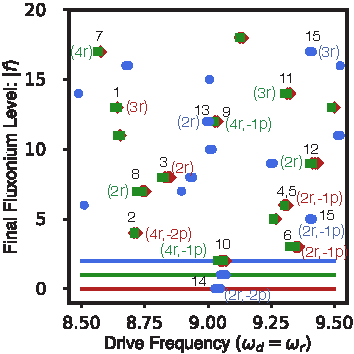
\includegraphics[width=\linewidth]{Figures/Trans_.pdf}
    \caption{{\bf Energy conserving processes $\ket{\tilde{i},\tilde{0}}\leftrightarrow\ket{\tilde{f},\tilde{y}}$ for Eq.~\ref{eq:En_cons} with $x\le 4, y\le 2, f\le 20$ and $i=0$ (red diamonds), $i=1$ (green squares), $i=2$ (blue circles).} The horizontal lines indicate the initial state $i$ for visual aid. Labels in black correspond to transition $\#$ listed in Table~\ref{tab:PMIST}. The colored labels correspond to the disjoint subspaces for simplified representation, but the energy conservation uses the eigen-energies of the hybridized eigenstates of $H_{0}$ (see Eq.~\ref{eq:bare_ham}). For example, the green label ($4 \mathrm{r},-1 \mathrm{p}$), for transition $8$ of Table~\ref{tab:PMIST}, shows the number of readout photons absorbed ($4$) and the number of parasitic mode ($\mu=2$) photons emitted ($1$) in the process. The faded points are weaker transitions not captured in the Floquet simulations.
}
    \label{fig:trans_prof}
\end{figure}

Fig.~\ref{fig:trans_prof} depicts all four-photon processes that occur with approximate energy conservation, for drive frequencies within our target range, and when starting in one of the four lowest fluxonium levels. The results from Floquet simulations are shown in solid dots and labeled in black (see Sec.~\ref{sec:MIST}), while the processes not identified in the simulation are faded. Note that there are downward transitions from $\ket{2}_\phi$ (blue dots) to the states $\ket{1}_\phi$ (green line) and $\ket{0}_\phi$ (red line) in the fluxonium subspace in the presence of parasitic modes. An example is captured by transition $14$ of Table~\ref{tab:PMIST}.

The parenthesized labels in color denote the number of readout photons ($x \mathrm{r}$) and parasitic mode photons ($y\mathrm{p}$) required for the transition in the fluxonium subspace, where a positive index denotes absorption/de-excitation while a negative index denotes emission/excitation. For example, transition $2$ corresponds to the emission of four readout photons, which are converted into two parasitic mode photons, absorbed by the mode $\mu=2$, as well as an excitation from $\ket{0}_\phi$ to $\ket{4}_\phi$ in the fluxonium subspace.

Intuitively, many readout photons are required to bridge a large energy gap between the readout frequency and parasitic mode frequency. As this gap increases, the likelihood of PMIST processes decreases. We verify this intuition by considering the dependence on both the parasitic mode frequency and drive frequency in what follows.

\paragraph{Parasitic Mode Frequency:}
An approach towards mitigating PMIST processes is to adjust $\omega_\mu$ so that $\omega_\mu \gg \omega_\textrm{r}$ for $\mu=2$, requiring more readout photons to be absorbed in PMIST processes and therefore reducing PMIST transition rates. The dependence of the parasitic mode frequencies for even $\mu$ is
\begin{align}
    \frac{\omega_\mu^\textrm{e}}{2\pi}&=\sqrt{8E_{\textrm{c},\mu}^\textrm{e} E_{\textrm{J}_\textrm{j}}}
\end{align}
See Eq.~\ref{eq:parasitic} for $E_{\textrm{c},\mu}^\textrm{e}$ and Table~\ref{tab:circuit_params} for $E_{\textrm{J}_\textrm{j}}$. Again, we focus on the large $N$ and small $\mu$ limit to focus on parasitic modes with the strongest coupling to the qubit. From derivations in Ref.~\cite{viola2015collective} it is clear that parasitic frequency decreases with an increase in junction count and parasitic ground capacitance. Thus, decreasing parasitic ground capacitance decreases both parasitic frequency and qubit-parasitic coupling. Increasing $N$, on the other hand, is only favorable for reducing the coupling strength while decreasing the gap between $\omega_\textrm{d}$ and $\omega_\mu$. The impact of decreasing $N$ to increase this gap would require consideration of nonlinear corrections as well as fixed inductance, thus making these changes difficult in practice~\cite{viola2015collective}.

\paragraph{Drive Frequency ($\omega_\textrm{d}$):} If, on the other hand, readout ($\omega_\textrm{d} \ll \omega_{\mu = 2}$), a large readout photon number $x$ would be needed while having a similar impact. We give the Floquet figure corresponding to a low-frequency readout regime in Fig.~\ref{fig:Flo_low}, which shows higher parasitic mode populations compared to our previous case in Fig.~\ref{fig:Floquet}. The PMIST effects can be explained by examining the increased density of resonances when $\omega_\textrm{d}/2\pi \approx 6 \ \mathrm{GHz}$. Note that this frequency is approximately the fluxonium plasma frequency $\omega_{12}/2\pi$ and is also half the parasitic mode $\mu=2$ frequency. This introduces multiple frequency collisions, which cause the various transitions observed in the figure. This logic already indicates that $5.5-6 \ \mathrm{GHz}$~\footnote{Further lower $\omega_\textrm{d}$ for readout is not favorable due to thermal heating of the readout resonator leading to photon-shot-noise induced dephasing of the qubit, and hence not analyzed in this work.} would be a bad range of frequencies for the current choice of parameters. Formal transition probability calculations, same as Sec.~\ref{sec:LZ}, will be required to predict how detrimental these effects can be. However, the energy conservation indicates that in spite of the increase in the number of PMIST effects, such transitions will be higher-order processes (large $x$) and thus suppressed for typical readout powers where $\bar n_\textrm{r}\sim \mathcal{O}(10^2)$~\cite{gusenkova2021quantum}.

\begin{figure}[t]
    \centering
    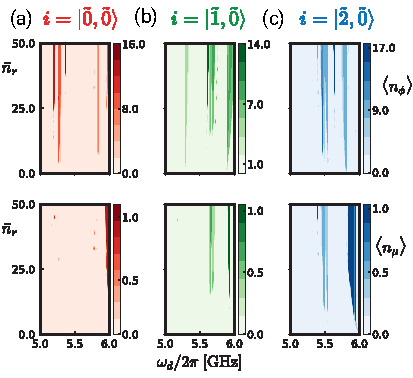
\includegraphics[width=\linewidth]{Figures/Floquet_low.pdf}
    \caption{{\bf Floquet simulations at lower readout frequencies.} Circuit parameters used are the same as quoted in Tables~\ref{tab:circuit_params} and~\ref{tab:readout_params} for branch analysis starting in the dressed hybridized eigenstate $i=\ket{\tilde{k},\tilde{0}}$, with maximum overlap to the un-hybridized states $\ket{k}_\phi\otimes\ket{0}_{\mu=2}$. The figures are plotted in linear scale, unlike Fig.~\ref{fig:Floquet}, making any streaks due to significantly weaker transitions unnoticeable.}
    \label{fig:Flo_low}
\end{figure}

A high-frequency readout $(\omega_\textrm{d}\gg \omega_{\mu=N-1})$ case requires a large Hilbert space and is beyond the scope of this work~\footnote{If $\omega_\textrm{d}\gg \omega_{\mu=N-1}$, a dominating transition mechanism for PMIST would correspond to an excitation of a strongly coupled, low-frequency parasitic mode (i.e., $\mu=\{2,4,6\}$) to a large photon number $y$, leaving just enough energy to produce excitation to some state $f$ in the fluxonium subspace of significant charge matrix elements (see Fig.~\ref{charge-matrix}). However, such large excitations in the parasitic modes would occur with lower probability because of the high photon number $y$ involved in the transition.}.

\subsection{Alternative circuit parameters}\label{Will_circuit}

Our analysis of PMIST so far has focused on systems where the fluxonium qubit frequency is $\omega_{01} / 2 \pi \sim 30$ MHz. Here, we consider how these processes change when one uses a larger qubit frequency $\omega_{01}/2\pi \sim 300 \ \mathrm{MHz}$, as was recently realized in the experiment of Ref.~\cite{ding_high-fidelity_2023} (see App.~\ref{app:alt_circuit1} for full circuit parameters). The parasitic mode frequency of the $\mu=2$ mode is $\omega_{\mu=2}/2\pi=15.50 \ \mathrm{GHz}$. The coupling strengths are: $g_{\phi \textrm{r}}/2\pi=37 \ \mathrm{MHz}$, $g_{\phi\mu}/2\pi=216 \ \mathrm{MHz}$, $g_{\mu \textrm{r}}/2\pi=6 \ \mathrm{MHz}$. The plasma frequency is $\omega_{12}/2\pi=5.40 \ \mathrm{GHz}$. The assumptions for numerical modeling are the same as previous Floquet simulations as discussed in App.~\ref{app:numerics}. Even though the coupling strengths for these circuit parameters are similar to our previous parameter set in Table~\ref{tab:readout_params}, since the $\mu=2$ parasitic mode is larger by about $4 \ \mathrm{GHz}$, we expect fewer PMIST processes for the drive frequency range analyzed in Fig.~\ref{fig:Floquet}.

\begin{figure}[t]
    \centering
    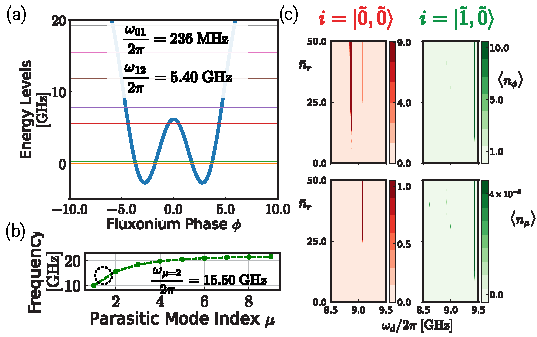
\includegraphics[width=\linewidth]{Figures/Floquet_Will.pdf}
    \caption{{\bf Floquet analysis with alternate JJA fluxonium parameters inspired by Ref.~\cite{ding_high-fidelity_2023}.} \textbf{(a)} Fluxonium energy spectrum. \textbf{(b)} Parasitic mode frequencies. \textbf{(c)} Floquet simulations for the branch analysis of the computational states. Circuit parameters for this circuit are discussed in Sec.~\ref{Will_circuit} and App.~\ref{app:alt_circuit1}. The Floquet figures are plotted in linear scale, unlike Fig.~\ref{fig:Floquet}, making any streaks due to significantly weaker transitions unnoticeable.}
    \label{fig:Floquet1}
\end{figure}

Fig.~\ref{fig:Floquet1} shows that indeed, PMIST effects are comparatively less likely for this alternate circuit. The single PMIST process observed in the Floquet profile $\ket{\tilde{0},\tilde{0}}\leftrightarrow\ket{\tilde{4},\tilde{1}}$ occurs at $\bar n_\textrm{r}=25$ and has the quasi-energy gap of $\Delta_\textrm{ac}=0.13 \ \mathrm{MHz}$ at the avoided crossing. The quasi-energy gap at the avoided crossing for this transition is $\Delta_\textrm{ac}=0.12$ MHz. The explicit transitions with quasi-energies for the Floquet profile shown in Fig.~\ref{fig:Floquet1}(c) can be found in App.~\ref{app:alt_circuit1}. The overall reduced number of MIST effects in Fig.~\ref{fig:Floquet1} compared to Fig.~\ref{fig:Floquet} is due to the fact that the charge matrix $|\bra{i}\hat H\ket{f}|^2$ elements between levels $i=0$ (and $i=1$) and higher fluxonium states ($f$) decrease faster with increasing $f$ for this circuit (compare Fig.~\ref{fig:charge-matrix-Will} with Fig.~\ref{charge-matrix}).

While the above results are promising, we stress that our analysis here considers a single specific PMIST process (i.e., involving the lowest-frequency array mode with the strongest qubit-parasitic coupling). Other less obvious processes may also play a role, for example, PMIST due to parasitic modes $\mu=4,6,\ldots$. The Floquet simulation including all relevant parasitic modes will be numerically intractable and hence warrants practical alternatives.

\section{Conclusion and Further Work}\label{sec:conclusion}
In this work, we have analyzed the impact of internal array degrees of freedom on driven JJA fluxonium qubits, showing that new pathways for measurement-induced state transitions can occur via excitations of JJA parasitic modes. These processes, which we have called PMIST, occur at particular resonance conditions when the energy of several readout photons is equal to a small number of parasitic mode excitations and a fluxonium mode excitation.

We find that PMIST transitions can occur at meaningfully high rates (with avoided crossing quasi-energy gap $\Delta_{\textrm{ac}}=0.66 \ \textrm{MHz}$) because of the strong coupling between parasitic modes and the qubit. As a result, such state transitions can occur even at low readout drive powers (corresponding to small intracavity photon numbers) while using typical parameters that enable high-fidelity, dispersive readout. For example, we have shown that PMIST does lower the onset of MIST processes to $\sim 10$ readout photons at certain drive frequencies. In addition, PMIST has the potential to significantly dephase the qubit post-measurement. This could in turn limit the qubit gate fidelities required for quantum error correction and ultimately the performance of a quantum processor. However, the coupling of the parasitic mode to the readout is still sufficiently weak such that, for the vast majority of readout frequencies, the JJA mode excitation population is negligible unless a PMIST occurs. \AC{I find the previous sentence quite confusing, don't know how to reword as I'm not sure what the point is you are trying to make.  Also seems to contradict the start of the paragraph, where you discuss ``strong coupling of the parasitic mode and the qubit".  Can you try to rephrase?} \sh{I agree with Aash. This sentence was addd by Emma in the spirit that there exist some frequencies for which PMIST will most likely not occur. However, it is indeed confusing. @Emma, can we remove or change this sentence please?} Therefore, these processes can be avoided via judicious choice of readout, junction array, and fluxonium parameters. We analyze the trend in PMIST for various drive frequencies, parasitic mode frequencies, coupling constants, and circuits with two different qubit frequencies equal to $\sim 30$ and $\sim 300 \ \mathrm{MHz}$.


We have presented a first analysis toward understanding the role of parasitic modes in the dispersive readout dynamics of a fluxonium circuit. Mitigating the parasitic mode excitations could involve careful selection of the readout resonator frequency and varying junction energies along the array to localize parasitic modes. Such modifications alter the parasitic mode spectrum towards reducing excitation probability. The circuit parameters used in this work correspond to a parasitic mode of the fluxonium's junction array. However, other modes with similar frequencies may also participate in the environment of the fluxonium. This may include, for example, confined package modes, slot line modes, and harmonics of coplanar waveguide resonators for readout. Our results show the significance of taking all such modes into consideration when driving many excitations into highly nonlinear circuits.

\section{Acknowledgments}
 We thank Akshay Koottandavida, Daniel K. Weiss, Sumeru Hazra, Alessandro Miano, Connor Hann, Kyungjoo Noh, Simon Leiu and Vidul R. Joshi for fruitful discussions. We are grateful to Simone Severini, Bill Vass, Oskar Painter, Fernando Brand\~ao, Eric Chisholm, and AWS for supporting the quantum computing program. %SS acknowledges support from the Army Research Office (ARO) under Grant Number W911NF-23-1-0051 for the time she spent on this project at Yale University. SS is grateful to Connor Hann for inviting her to pursue an internship program at AWS where this project started.
\appendix
\section{Role of symmetry in readout circuits}\label{app:alt_circuits}
\begin{figure}[t]
    \centering
    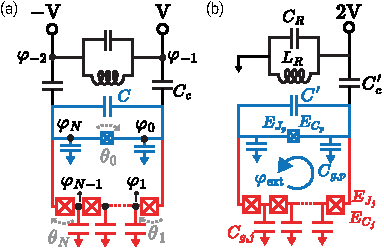
\includegraphics[width=\linewidth]{Supp_Fig/Circuit_choice.pdf}
    \caption{{\bf Alternative readout circuits.} (a) Symmetric circuit same as Fig.~\ref{fig:meas_circuit}(a), (b) Asymmetric circuit inspired by Ref.~\cite{zhang_universal_2021}. Alternative (b) requires a single-point connection to the readout line, unlike the symmetric circuit in (a). The symmetric circuit is used as a reference for denoting phase variables $\varphi_i$ at each node and phase difference variables $\theta_j$ across each junction used in the derivation of the Lagrangian for both circuits.}
    \label{fig:circuit_choice}
\end{figure}

\begin{table}[htb]
    \begin{center}
    \begin{tabular}{|c |c| c |c| }
     \hline
     \textbf{Parameters} & \textbf{Variables} & \textbf{Values}\\ 
    \hline
    Phase-slip JJ capacitance &$\textrm{C}_\textrm{p}$ &$13.3$ fF\\ 
    \hline
    Differential capacitance &$C$ &$1.14$ fF\\ 
    \hline
    JJA capacitance energy&$\textrm{C}_\textrm{j}$&$26.2$ fF\\ 
    \hline
    JJA ground capacitance&$C_\textrm{g,j}$&$0.1 \ \mathrm{fF}$\\ 
    \hline
    Phase-slip ground capacitance&$C_\textrm{g,p}$&$10 \ \mathrm{fF}$\\ 
    \hline
    Coupling capacitance&$C_\textrm{c}$ &$1 \ \mathrm{fF}$\\ 
     \hline
      ZPF of the resonator/drive&$V_{\mathrm{ZPF}}$&$0.75$ GHz\\
     \hline
      ZPF of fluxonium charge operator&$N_{\phi,\mathrm{ZPF}}$&$0.36$\\
     \hline
      ZPF of parasitic charge operator&$N_{\mu=2,\mathrm{ZPF}}$&$1.58$\\
     \hline
    \end{tabular}
    \end{center}
    
    \caption{{\bf Capacitances and zero-point fluctuation (ZPF) values.} These circuit parameters are used throughout this article.}
    \label{tab:params}
    \end{table}
    The fluxonium readout circuit in Fig.~\ref{fig:meas_circuit} can be modified in several ways, affecting performance metrics. This circuit has a symmetric configuration with a symmetry (identified in Ref.~\cite{ferguson2013symmetries}) that removes coupling to the lowest frequency mode $\mu=1$~\cite{viola2015collective}. Crucial to this symmetry are the equal coupling capacitances on both ends of the circuit (see Fig.~\ref{fig:circuit_choice}(a)). We present a modification with a different grounding option that does not respect this symmetry (see Fig.~\ref{fig:circuit_choice}(b)). This asymmetric circuit, inspired by~\cite{zhang_universal_2021}, is useful in a hangar geometry with a single voltage line. In this appendix, we derive the Lagrangian for both circuits and show that not preserving this symmetry can be detrimental for readout. Therefore, we use the symmetric circuit for readout in the rest of the appendix and the main text.
\subsection{Lagrangian}

To derive the Lagrangians, we follow the recipe in Refs.~\cite{viola2015collective,ferguson2013symmetries} for the symmetric circuit and adapt it for the asymmetric circuit in Fig.~\ref{fig:circuit_choice}(b). Importantly, we show that the symmetry in the circuit, which prevents any coupling with the lowest-frequency parasitic mode ($\mu=1$), is not preserved in the asymmetric circuit. The presence of coupling to this mode is detrimental for readout, as discussed in Sec.~\ref{sec:expressions}.

The Lagrangian corresponding to both circuits is a combination of the Lagrangians, $\mathcal{L}_\textrm{phase-slip}$ from the phase-slip junction shown in blue (comprising of the junction with $E_{\textrm{J}}/E_{\textrm{C}}\sim 5-8$ and the capacitor $C$), $\mathcal{L}_\textrm{JJA}$ from the (red) junctions in the array, $\mathcal{L}_\textrm{g}$ from the ground capacitances, $\mathcal{L}_\textrm{R}$ from the readout resonator and $\mathcal{L}_\textrm{c}$ due to the coupling capacitances $C_\textrm{c}$. The node flux variables at various points in the circuit are denoted by $\varphi_i=2\pi\Phi_i/\Phi_0$. We mark the phase-difference across the junctions in the array, $\theta_{i}=\varphi_i-\varphi_{i-1}$, and across the phase-slip junction, $\theta_0=\varphi_\textrm{N}-\varphi_{0}$, as shown in Figs.~\ref{fig:circuit_choice}(b,c). Similarly, the voltage drop across each junction is given by the phase evolution equation $\dot{\theta}_i=\dot{\varphi}_i-\dot{\varphi}_{i-1}=2\pi V_i/\Phi_0$ where $\Phi_0=h/2e$ the superconducting flux quantum. We will use subscripts $\textrm{j, p}$ for JJA and the phase-slip junction coordinates, respectively. For the Lagrangian of the symmetric circuit~\cite{viola2015collective,ferguson2013symmetries} (setting $\hbar=1$), we have, 
\begin{align}
    \mathcal{L}&=\mathcal{L}_{\textrm{phase-slip}}+\mathcal{L}_{\textrm{JJA}}+\mathcal{L}_{\textrm{g}}+\mathcal{L}_{\textrm{R}}+\mathcal{L}_{\textrm{C}},
\end{align}
where
\allowdisplaybreaks{
\begin{align}
    \mathcal{L}_{\textrm{phase-slip}}&=\frac{1}{16E_{\textrm{C}}}(\dot{\varphi_\textrm{N}}-\dot{\varphi_0})^2-E_{\textrm{J}_\textrm{p}}\cos\big(\sum_{i=1}^N\theta_i+\varphi_\mathrm{ext}\big)\\
    \mathcal{L}_{\textrm{JJA}}&=\sum_{i=1}^N\frac{1}{16E_{\textrm{C}_\textrm{j}}}(\dot{\varphi}_i-\dot{\varphi}_{i-1})^2-E_{\textrm{J}_\textrm{j}}\cos(\theta_i)\\
    \mathcal{L}_\textrm{R}&=\frac{1}{16E_{C_\textrm{R}}}(\dot{\varphi}_{-1}-\dot{\varphi}_{-2})^2+\frac{1}{16E_{\textrm{L}_\textrm{R}}}(\varphi_{-1}-\varphi_{-2})^2\\
    \mathcal{L}_{\textrm{g}}&=\sum_{i=1}^{N-1} \frac{\dot{\varphi_i}^2}{16E_{\textrm{g,j}}}+\sum_{i=0,N} \frac{\dot{\varphi_i}^2}{16E_{\textrm{g,p}}}\\
    \mathcal{L}_{\textrm{c}}&=\frac{1}{16E_{\textrm{c}}}(\dot{\varphi}_{-1}-\dot{\varphi_0})^2+\frac{1}{16E_{\textrm{c}}}(\dot{\varphi}_{-2}-\dot{\varphi}_\textrm{N})^2\nonumber\\
    &=\frac{\dot{\varphi}^2_0}{16E_{\textrm{c}}}+\frac{\dot{\varphi}^2_{-1}}{16E_{\textrm{c}}}-\frac{\dot{\varphi}_0\dot{\varphi}_{-1}}{8E_{\textrm{c}}}\nonumber\\&\quad+\frac{\dot{\varphi}^2_\textrm{N}}{16E_{\textrm{c}}}+\frac{\dot{\varphi}^2_{-2}}{16E_{\textrm{c}}}-\frac{\dot{\varphi}_\textrm{N}\dot{\varphi}_{-2}}{8E_{\textrm{c}}}.\label{eq:float-float}
\end{align}
}
The definitions and values of capacitive energies used here are given in Table~\ref{tab:circuit_params} for the symmetric circuit. The terms associated with $\dot{\varphi}_i (\theta_i)$ are the kinetic (potential) energy terms. We can ignore the harmonic oscillator Lagrangian $\mathcal{L}_\textrm{R}$ due to triviality. Note that for the asymmetric floating fluxonium and grounded fluxonium circuits (see Figs.~\ref{fig:circuit_choice}(b,c)), we can respectively impose $\dot{\varphi}_{-2}=0$ and $\dot{\varphi}_{\textrm{N}}=0$. First, we expand on the derivation in Refs.~\cite{ferguson2013symmetries,viola2015collective} for completeness and then impose these conditions to derive the Lagrangians for all three cases.

We use the definition of phase difference quadratures and the fluxoid quantization with an external flux choice of $\varphi_{\mathrm{ext}}=\pi$ as per the main text.
\begin{align}
\sum_{l=1}^m\theta_l&=\varphi_m-\varphi_0\\
\sum_{m=0}^N \theta_m+\varphi_\mathrm{ext}&=2\pi z,
\end{align}
where $z\in\mathbb{Z}$. Writing the the Lagrangian in this new basis follows $\partial \mathcal{L}/\partial \dot{\varphi}_0=0$ yields the expression,
\begin{align}
\dot{\varphi}_0&=E_{\textrm{t}}\Big(\frac{\dot{\varphi}_{-1}}{E_{\textrm{c}}}+\frac{\dot{\varphi}_{-2}}{E_{\textrm{c}}}-\sum_{l=1}^{N}\frac{\dot{\theta}_l}{E_{\textrm{c}}}-\sum_{l=1}^{N}\frac{\dot{\theta}_l}{E_{\textrm{g,p}}}\nonumber\\&\quad-\sum_{i=1}^{N-1}(N-i)\frac{\dot{\theta}_i}{E_{\textrm{g,j}}}\Big)
\end{align}
where
\begin{align}
E_\textrm{t}=\Big(\frac{2}{E_{\textrm{c}}}+\frac{N-1}{E_{\textrm{g,j}}}+\frac{2}{E_{\textrm{g,p}}}\Big)^{-1}\label{eq:tot_cap}
\end{align}
is the total capacitive energy of the circuit due to the parasitic ground capacitances and coupling capacitances. Using the expression for $\dot{\varphi}_0$, we get $\mathcal{L}_\textrm{c}+\mathcal{L}_\textrm{g}=$,
\begin{align}
&\frac{\big(\dot{\varphi}^2_{-1}+\dot{\varphi}^2_{-2}\big)}{16E_\textrm{c}}\Big(1-\frac{E_\textrm{t}}{E_\textrm{c}}\Big)+\frac{\dot{\varphi}_{-1}\dot{\varphi}_{-2}}{8E_\textrm{c}}\Big(\frac{E_\textrm{t}}{E_\textrm{c}}\Big)\nonumber\\
&+\sum_{i=1}^N\Big(\frac{\dot{\varphi}_{-1}\dot{\theta}_i}{E_\textrm{c}}+\frac{\dot{\varphi}_{-2}\dot{\theta}_i}{E_\textrm{c}}\Big)\Big(\frac{E_\textrm{t}}{8E_\textrm{c}}+\frac{E_\textrm{t}}{8E_\textrm{g,p}}\Big)\nonumber\\&+\sum_{i=1}^{N-1}\Big(\frac{\dot{\varphi}_{-1}\dot{\theta}_i}{E_\textrm{c}}+\frac{\dot{\varphi}_{-2}\dot{\theta}_i}{E_\textrm{c}}\Big)\frac{(N-i)E_\textrm{t}}{8E_\textrm{g,j}}\nonumber\\
&-\sum_{i=1}^N\frac{\dot{\varphi}_{-2}\dot{\theta}_i}{8E_\textrm{c}}+\Big(\sum_{i=1}^N\dot{\theta}_i\Big)^2\Bigg(\frac{1}{16E_\textrm{c}}+\frac{1}{16E_\textrm{g,p}}\Bigg)\nonumber\\&\quad\times\Bigg(1-\frac{E_\textrm{t}}{E_\textrm{c}}-\frac{E_\textrm{t}}{E_\textrm{g,p}}\Bigg)+\frac{\sum_{i=1}^{N-1}\big(\sum_{l=1}^i\dot{\theta}_l\big)^2}{16E_\textrm{g,j}}\nonumber\\
&-2\sum_{l=1}^N \sum_{l'=1}^{N-1}\dot{\theta}_l\dot{\theta}_{l'}(N-l')\Bigg(\frac{E_\textrm{t}}{8E_\textrm{c}E_\textrm{g,j}}+\frac{E_\textrm{t}}{8E_\textrm{g,p}E_\textrm{g,j}}\Bigg)\nonumber\\
&-\frac{E_\textrm{t}}{16}\Bigg[\frac{\sum_{i=1}^{N-1}(N-i)\theta_i}{E_\textrm{g,j}}\Bigg]^2.
\end{align}
\sh{Start spell check here.}
We will eventually use the scalar voltage values for $\dot{\varphi}_{-1},\dot{\varphi}_{-2}$ and hence we can ignore any term solely dependent on these variables. The terms independent of $\dot{\varphi}_{-1},\dot{\varphi}_{-2}$ are combined as $\sum_{l=1}^{N}\sum_{l=1}^{N}\mathcal{G}_{ll'}\dot{\theta}_l\dot{\theta}_{l'}$ where,
\begin{align}
\mathcal{G}_{ll'}&=\Big[\frac{\textrm{N}-\text{max}\{l,l'\}}{16E_\textrm{g,j}}+\frac{1}{16E_\textrm{c}}+\frac{1}{16E_\textrm{g,p}}\Big]\nonumber\\&\quad\times\Big[1-\frac{E_\textrm{t}}{E_\textrm{c}}-\frac{E_\textrm{t}}{E_\textrm{g,p}}-(\textrm{N}-\text{min}\{l,l'\})\frac{E_\textrm{t}}{E_\textrm{g,j}}\Big]
\end{align}
This final expression matches with Refs.~\cite{ferguson2013symmetries,viola2015collective}, for an ordered array.
\subsection{Collective modes.} 
Now, we will define the collective modes for the fluxonium circuit, $\{\phi,\xi_1,...,\xi_{\textrm{N}-1}\}$ such that 
\begin{align}
    \theta_m=\phi/N+\sum_\mu W_{\mu m}\xi_\mu,
\end{align}
and inversely,
\begin{align}
    \phi&=\sum_{m=1}^N\theta_m,\quad \xi_\mu=\sum_{m=1}^N W_{\mu m}\theta_m.
\end{align}
Here, $\phi$ is called the superinductance mode or the \emph{qubit} mode while $\xi_\mu$ denote the parasitic modes indexed by $\mu\in\{1,..,N-1\}$~\cite{ferguson2013symmetries}. The matrix $W$ is semi-orthogonal, with dimensions $(N-1)\times N$, and is given by $\sum_m W_{\mu m}W_{\nu m}=\delta_{\mu \nu}$. Its row sum is zero, $\sum_mW_{\mu m}=0$. Thus, the following choice
\begin{align}
    W_{\mu m}=\sqrt{\frac{2}{N}}\cos{\frac{\pi\mu(m-1/2)}{N}},
\end{align}
is observed in~\cite{ferguson2013symmetries} and later used in~\cite{viola2015collective} to derive the Hamiltonian for the symmetric circuit.
The choice of these new variables highlights the collective modes describing the low-energy physics as illustrated in~\cite{catelani2011relaxation,koch2009charging,manucharyan2009fluxonium}. We can now split the combined Lagrangian $\mathcal{L}=\mathcal{T}-\mathcal{U}$ into kinteic energy $\mathcal{T}$ and potential energy $
\mathcal{U}$ terms in the basis of collective modes as,
\begin{align}
\mathcal{T}=&\Big[\Big(\frac{\dot{\varphi}_{-1}}{E_{\textrm{c}}}+\frac{\dot{\varphi}_{-2}}{E_{\textrm{c}}}\Big)\Big(\frac{E_{\textrm{t}}}{8E_{\textrm{c}}}+\frac{E_{\textrm{t}}}{8E_{\textrm{g,p}}}\Big)-\frac{\dot{\varphi}_{-2}}{8E_{\textrm{c}}}\Big]\dot{\phi}\nonumber\\&+\sum_{l=1}^{N-1}(N-l)\frac{E_{\textrm{t}}}{8E_{\textrm{g,j}}}\Big(\frac{\dot{\varphi}_{-1}}{E_{\textrm{c}}}+\frac{\dot{\varphi}_{-2}}{E_{\textrm{c}}}\Big)\Big](\dot{\phi}/N+\sum_\mu W_{\mu l}\dot{\xi}_\mu)\nonumber\\
  &+\sum_{l=1}^N\sum_{l'=1}^N(\dot{\phi}/N+\sum_\mu W_{\mu l}\dot{\xi}_\mu)(\dot{\phi}/N+\sum_\mu W_{\mu l'}\dot{\xi}_\mu)\nonumber\\
  &\times\Big[\frac{\textrm{N}-\text{max}\{l,l'\}}{16E_\textrm{g,j}}+\frac{1}{16E_\textrm{c}}+\frac{1}{16E_\textrm{g,p}}\Big]\nonumber\\&\times\Big[1-\frac{E_\textrm{t}}{E_\textrm{c}}-\frac{E_\textrm{t}}{E_\textrm{g,p}}-(\textrm{N}-\text{min}\{l,l'\})\frac{E_\textrm{t}}{E_\textrm{g,j}}\Big]\label{eq:kin-energy}\\
    \mathcal{U}&=-E_{\textrm{J}_\textrm{p}}\cos(\phi)-\sum_{l=1}^NE_{\textrm{J}_\textrm{j}}\cos\Big(\phi/N+\sum_\mu W_{\mu l}\xi_\mu\Big)\label{eq:pot-energy}
\end{align}
\subsection{Circuit modifications and assumptions}
From here on, we define a sum over $m,n$ as running from $1$ to $N$, while the sum over $\mu,\nu$ runs from $1$ to $N-1$. In order to simplify the Lagrangian for the different circuits, we will recall that $\sum_m W_{\mu m}=0$, and the semi-orthogonal matrix condition $\sum_m W_{\mu m}W_{\nu m}=\delta_{\mu\nu}$, yielding the identities,
\begin{align}
 \sum_{n=1}^m W_{\mu n}&=-\sum_{n=m+1}^N W_{\mu n}\\
 \sum_{m=1}^N mW_{\mu m}&=-\frac{c_\mu o_{\mu}}{\sqrt{2N}s_\mu^2}\\
 \sum_{m=1}^N m^2W_{\mu m}&=\frac{c_\mu}{\sqrt{2N}s_\mu^2}[N(-1)^\mu-o_\mu]
\end{align}
where $o_\mu=\frac{[1-(-1)^\mu]}{2},c_\mu=\cos{\frac{\pi\mu}{2N}}, s_\mu=\sin{\frac{\pi\mu}{2N}}$. We will now simplify the kinetic energy and potential energy terms from Eqs.~\ref{eq:pot-energy} and~\ref{eq:kin-energy}, for the different circuits, using these identities.
\paragraph{Linear Approximation}
We discuss the simplification under linear assumption on the parasitic modes $\mu$. This includes only linear terms from Taylor expansion of the cosine ($\cos{x}\sim 1-\frac{x^2}{2}$) Eq.~\ref{eq:pot-energy}, yielding (up to a constant term)
\allowdisplaybreaks{
\begin{align}
    \mathcal{U}&=E_{\textrm{J}_\textrm{p}}\cos(\phi)+\frac{E_{\textrm{J}_\textrm{j}}}{2N}\phi^2+\frac{E_{\textrm{J}_\textrm{j}}}{2}\sum_{\mu}\xi_\mu^2\\
    &=E_{\textrm{J}_\textrm{p}}\cos(\phi)+\frac{E_{\textrm{J}_\textrm{j}}}{2N}\phi^2+\frac{E_{\textrm{J}_\textrm{j}}}{2}\sum_{\mu}\xi_\mu^2,
    \end{align}
}

 The potential energy of both circuits remains the same ($\mathcal{U}=\mathcal{U}_1=\mathcal{U}_2$). 
\paragraph{Symmetric circuit.} For the circuit in Fig.~\ref{fig:circuit_choice}(a), let the Lagrangian be denoted by $\mathcal{L}_1=\mathcal{T}_1-\mathcal{U}_1$ and impose the conditions $\dot{\varphi}_{-1}=2\textrm{eV},\dot{\varphi}_{-2}=-2\textrm{eV}$.
    \begin{align}
\mathcal{T}_1&=-\frac{\dot{\phi}\textrm{eV}}{4E_{\textrm{c}}}+\Big[(M_{00}+G_{00})\dot{\phi}^2+2\sum_{\mu}(M_{0\mu}\nonumber\\&\quad+G_{0\mu})\dot{\phi}\dot{\xi_\mu}+\sum_{\mu,\nu}(M_{\mu\nu}+G_{\mu\nu})\dot{\xi_\mu}\dot{\xi_\nu}\Big].\end{align}
Here $M$ comes from the phase-slip junction and JJA while $G$ comes from the coupling and ground capacitances, and these coefficients are given by,
\begin{align}
M_{00}&=\frac{1}{E_{C_\textrm{tot}}}+\frac{1}{NE_{\textrm{C}_\textrm{j}}}, M_{0\mu}=0,    M_{\mu\nu}=\frac{\delta_{\mu\nu}}{E_{\textrm{C}_\textrm{j}}}\\
G_{00}&=\frac{1}{64E_{\textrm{t}}}\Big[1-\frac{2}{3}\frac{(N^2-1)E_\textrm{t}}{NE_\textrm{g,j}}\Big]\\
G_{0\mu}&=-\frac{c_\mu o_{\mu+1}}{32E_{\textrm{g,j}}\sqrt{2N}s_\mu^2}\\
G_{\mu\nu}&=\frac{1}{64E_{\textrm{g,j}}s_\mu^2}\Big[\delta_{\mu\nu}-\frac{E_{\textrm{t}}}{E_{\textrm{g,j}}}\frac{2c_\mu c_\nu o_\mu o_\nu}{N s_\nu^2}\Big].
\end{align}
Note that $C_\textrm{tot}=\textrm{C}_\textrm{p}+C$ is the total capacitance used for the qubit mode. The quantities $G_{00},G_{0\mu},G_{\mu\nu}$ contribute to the equations for the coupling strengths in the final Hamiltonian while $M_{00},M_{\nu\nu}$ contribute to the charging energies of the qubit and parasitic modes, discussed in Sec.~\ref{sec:expressions}. We can see that only the parasitic modes with even index $\mu$ interact with the qubit since $G_{0\mu}=0$ for $\mu\in 2\mathbb{Z}+1$. The Hamiltonian for the symmetric case, thus, will also not couple the odd modes (especially  parasitic mode $\mu=1$) with the qubit. 
\paragraph{Asymmetric circuit.} For the circuit in Fig.~\ref{fig:circuit_choice}(b), let the Lagrangian be denoted by $\mathcal{L}_2=\mathcal{T}_2-\mathcal{U}_2$ and impose the conditions 
$\dot{\varphi}_{-1}=4\textrm{eV},\dot{\varphi}_{-2}=0$. In addition $C_\textrm{c}=0$ on one end. The changes in the derivation include,
\begin{align}
\dot{\varphi}_0&=E_{\textrm{t}}\Big(\frac{\dot{\varphi}_{-1}}{E_{\textrm{c}}}-\sum_{l=1}^{N}\frac{\dot{\theta}_l}{E_{\textrm{g,p}}}-\sum_{i=1}^{N-1}(N-i)\frac{\dot{\theta}_i}{E_{\textrm{g,j}}}\Big)\\
E_\textrm{t}&=\Big(\frac{1}{E_{\textrm{c}}}+\frac{N-1}{E_{\textrm{g,j}}}+\frac{2}{E_{\textrm{g,p}}}\Big)^{-1}\\
\mathcal{L}_\textrm{c}&+\mathcal{L}_\textrm{g}
=\nonumber\\&\sum_{i=1}^N\frac{\dot{\varphi}_{-1}\dot{\theta}_i}{E_\textrm{c}}\Big(\frac{E_\textrm{t}}{8E_\textrm{g,p}}\Big)+\sum_{i=1}^{N-1}\frac{\dot{\varphi}_{-1}\dot{\theta}_i}{E_\textrm{c}}\frac{(N-i)E_\textrm{t}}{8E_\textrm{g,j}}\nonumber\\
&+\sum_{l=1}^{N}\sum_{l=1}^{N}\mathcal{G}_{ll'}\dot{\theta}_l\dot{\theta}_{l'},\\
\mathcal{G}_{ll'}&=\Big[\frac{\textrm{N}-\text{max}\{l,l'\}}{16E_\textrm{g,j}}+\frac{1}{16E_\textrm{g,p}}\Big]\nonumber\\&\quad\times\Big[1-\frac{E_\textrm{t}}{E_\textrm{g,p}}-(\textrm{N}-\text{min}\{l,l'\})\frac{E_\textrm{t}}{E_\textrm{g,j}}\Big]\\
%\mathcal{T}_2&=\Big[\frac{\textrm{eV}}{4E_\textrm{c}}\Big[\frac{2E_{\textrm{t}}}{E_{\textrm{g,p}}}+\frac{(N-1)E_{\textrm{t}}}{E_{\textrm{g,j}}}\Big]+(M_{00}'+G_{00}')\dot{\phi}\Big]\dot{\phi}\nonumber\\&-\Big[\frac{E_{\textrm{t}}}{2E_{\textrm{g,j}}E_{\textrm{c}}} \sum_\mu\frac{c_\mu o_\mu}{\sqrt{2N}s_\mu^2} \textrm{eV}-2(M_{0\mu}'+G_{0\mu}')\dot{\phi}\Big]\dot{\xi_\mu}\nonumber\\    &\quad+\sum_{\mu,\nu}(M_{\mu\nu}'+G_{\mu\nu}')\dot{\xi_\mu}\dot{\xi_\nu}\\
\mathcal{T}_2&=\frac{\dot{\phi}\textrm{eV}}{4E_\textrm{c}}\Big[1-\frac{E_\textrm{t}}{E_\textrm{c}}\Big]-\frac{E_{\textrm{t}}}{2E_{\textrm{g,j}}E_{\textrm{c}}} \sum_\mu\frac{c_\mu o_\mu}{\sqrt{2N}s_\mu^2} \dot{\xi_\mu}\textrm{eV}\nonumber\\&+(M_{00}+G_{00}')\dot{\phi}^2-2(M_{0\mu}+G_{0\mu}')\dot{\phi}\dot{\xi_\mu}\nonumber\\&+\sum_{\mu,\nu}(M_{\mu\nu}+G_{\mu\nu})\dot{\xi_\mu}\dot{\xi_\nu}\\
G_{00}'&=\frac{1}{64E_{\textrm{t}}}\Bigg[1-\frac{2}{3}\frac{(N^2-1)E_\textrm{t}}{NE_\textrm{g,j}}-\frac{2E_\textrm{t}}{E_\textrm{c}}\Bigg],\\
G_{0\mu}'&=-\frac{c_\mu}{32E_{\textrm{g,j}}\sqrt{2N}s_\mu^2}\Bigg[o_{\mu+1}-\frac{NE_\textrm{t}}{E_\textrm{c}}o_{\mu}\Bigg].
\end{align}
We can see that the parasitic modes with even and odd indices $\mu$ interact with the qubit as $G_{0\mu}'\neq 0\quad \forall\quad\mu$. The Hamiltonian for the symmetric case, thus, will also couple the odd modes (especially  parasitic mode $\mu=1$) with the qubit. 

The derived Lagrangians provide the Hamiltonians for each circuit. Ref.~\cite{viola2015collective} demonstrated that the symmetric circuit's Lagrangian, \( \mathcal{L}_1 \), under certain assumptions on \( N \), yields the Hamiltonian in Eqs.~\ref{Hamiltonian_total}-\ref{eq:int_hamiltonian}, where the coupling between the qubit and odd modes is zero. In contrast, we claim the asymmetric circuit's Lagrangian, \( \mathcal{L}_2 \), results in a Hamiltonian with non-zero couplings between the qubit and all parasitic modes (odd and even). Thus, the symmetric case eliminates coupling to certain parasitic modes, including the lowest-frequency mode (\( \mu = 1 \)), while the asymmetric case lacks this advantage. Given the parasitic frequency spectrum in Fig. \ref{fig:meas_circuit}(c) and the discussion in Sec.~\ref{sec:expressions}, the symmetric circuit's Floquet landscape is expected to exhibit fewer parasitic MISTs than the asymmetric circuit. Therefore, we focus exclusively on the symmetric circuit, as shown in Fig.~\ref{fig:meas_circuit}(c) and Fig.~\ref{fig:circuit_choice}(a) of the main text.


%\paragraph{Asymmetric grounded fluxonium circuit.} For the circuit in Fig.~\ref{fig:circuit_choice}(c), let the Lagrangian be denoted by $\mathcal{L}_3=\mathcal{T}_3-\mathcal{U}_3$ and impose the conditions 
%$\dot{\varphi}_{-1}=4\textrm{eV},\dot{\varphi}_{-2}=0,\dot{\varphi}_N=0$. In addition $C_\textrm{c}=0$ on one end. The changes in the derivation include,
%\begin{align}
%\mathcal{T}_3&=-\frac{(N+1)E_{\textrm{t}}}{16E_{\textrm{g}}E_{\textrm{c}}}\dot{\phi}\textrm{eV}-\frac{E_{\textrm{t}}}{8E_{\textrm{g}}E_{\textrm{c}}} \sum_\mu\frac{c_\mu o_\mu}{\sqrt{2N}s_\mu^2}  \dot{\xi}_\mu \textrm{eV}\nonumber\\
%&\quad+\Big[(M_{00}''+G_{00}'')\dot{\phi}^2+2\sum_{\mu}(M_{0\mu}''+G_{0\mu}'')\dot{\phi}\dot{\xi_\mu}\nonumber\\&\quad+\sum_{\mu,\nu}(M_{\mu\nu}''+G_{\mu\nu}'')\dot{\xi_\mu}\dot{\xi_\nu}\Big]. 
%\end{align}

\section{Undriven fluxonium circuit}\label{app:Hamiltonian}
In this appendix, we summarize the expressions for coupling strengths and charging energies used in Eqs.~\ref{Hamiltonian_total}-\ref{eq:int_hamiltonian}. We will analyze the effect of variations in circuit parameters on these quantities. This analysis is used in Sec~\ref{sec:expressions} to comment on the dependence of the parasitic effects captured in this work on circuit parameters. We also discuss the quantities related to the corresponding dispersive qubit Hamiltonians and give expressions for the dispersive coupling $\chi_{\phi\mu}$ used in Sec.~\ref{sec:dephasing}. Following the main text, we set $\hbar=1$. 

\subsection{Variation in charging energies and coupling strengths with circuit parameters}\label{app:coupling}
Here, we show the variations of the couplings and charging energies referenced in the main text, using the expressions derived in Ref.~\cite{viola2015collective}, with number of junctions $N$ and parasitic ground capacitance $C_\textrm{g,j}$, used in Sec.~\ref{sec:expressions}. \begin{figure}[tbh]
    \centering
    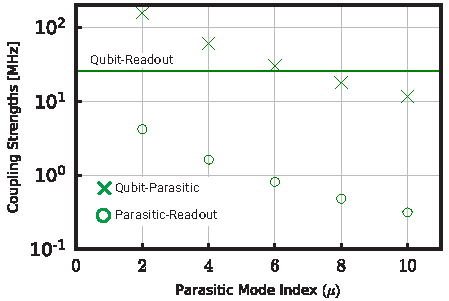
\includegraphics[width=\linewidth]{Supp_Fig/Coupling-strength.pdf}
    \caption{{\bf Absolute values of the coupling strengths.} $g_{\phi \textrm{r}}/2\pi$ (qubit-readout), $g_{\phi\mu}/2\pi$ (qubit-parasitic), $g_{\mu r}/2\pi$ (parasitic-readout), for various circuits. Coupling to odd parasitic modes is zero due to the symmetries of the circuit~\cite{viola2015collective}. The parasitic modes $\mu\in\{2,4,6\}$ couple to the qubit more strongly than the readout.}
    \label{fig:coupling-strength}
\end{figure}
\begin{enumerate}
\item Qubit Charging energy ($E_{\textrm{c}}^\phi \hat N_{\phi}^2$): The target qubit charging energy is affected by parasitic effects since $\frac{1}{E_\textrm{t}}\neq 0$.\\ $\frac{1}{\bar{E}_\textrm{c}^\phi}=\frac{1}{4E_{\textrm{t}}}\Big(1-\frac{2}{3}\frac{N^2-1}{N}\frac{E_{\textrm{t}}}{E_{\textrm{g,j}}}\Big)+\frac{1}{E_{\textrm{C}}}+\frac{1}{NE_{\textrm{C}_\textrm{j}}}$.
\item Even Parasitic Mode Charging Energy ($E_{\textrm{c},\mu}^\textrm{e}$): The parasitic charging energy is crucial in deciding the parasitic mode frequency $\omega_{\mu}$. And since only even parasitic modes (with index $\mu\in 2\mathbb{Z}$) couple to the qubit we will only give expressions for the even modes here.\\ $\frac{1}{\tilde{E}_{\textrm{c},\mu}^{e}}=\frac{1}{E_{\textrm{C}_\textrm{j}}}+\frac{1}{4E_{\textrm{g,j}}s_\mu^2}.$ 
\item Qubit-Readout Coupling ($g_{\phi \textrm{r}}$):\\ $g_{\phi \textrm{r}}=\frac{\tilde{E}_\textrm{c}^\phi}{E_{\textrm{c}}} N_{\phi,\mathrm{ZPF}}N_{\mu,\mathrm{ZPF}}.$
\item Qubit-Parasitic Coupling ($g_{\phi\mu}$): The coupling strengths as shown in Fig.~\ref{fig:coupling-Floquet} induce all MIST effects. In particular, the parasitic-qubit coupling $g_{\phi\mu}$ is responsible for PMIST effects.\\ $g_{\phi\mu}=\sqrt{\frac{2}{N}} \frac{\tilde{E}^\phi_\textrm{c}\tilde{E}^\textrm{e}_{\textrm{c},\mu}c_\mu}{E_{\textrm{g,j}}s_\mu^2} N_{\phi,\mathrm{ZPF}} N_{\mu,\mathrm{ZPF}}.$
\item Readout-Parasitic Coupling ($g_{\mu r}$): The parasitic-readout coupling $g_{\mu r}$ only increases population of the parasitic modes and is directly proportional to $g_{\phi\mu}$. We do not see any significant effects due $g_{\mu \textrm{r}}$ quantity in this work.\\ $g_{\mu r}=\frac{\tilde{E}^\phi_\textrm{c}\tilde{E}^\textrm{e}_{\textrm{c},\mu}c_\mu}{4\sqrt{2N}E_{\textrm{g,j}}E_{\textrm{c}}s_\mu^2} N_{\mu,\mathrm{ZPF}}N_{\textrm{r},\mathrm{ZPF}}.$   
\end{enumerate}

Fig.~\ref{fig:coupling-strength} shows that the lowest three even modes $\mu=2,4,6$ couple to the qubit stronger than the readout. This observation is a backbone of our work; we find that because of this relatively large coupling strength, PMIST rates may be significant in fluxonium-based quantum computers. In Fig.~\ref{fig:circuit_comp}, we show the dependence of charging energies and coupling constants on the number of junctions $N$ as well as the ground capacitance $C_\textrm{g,j}$. \footnote{Note that, the assumptions used in Ref.~\cite{viola2015collective} to derive the Hamiltonian was respected when analyzing the variation with $N$. } We focus on specifically on $g_{\phi\mu}$ and $E_{\textrm{c},\mu}^\textrm{e}$ because parasitic charging energy decides the parasitic frequency while the presence of qubit-parasitic coupling is the main culprit behind PMIST.

\begin{figure}[t]
    \centering
    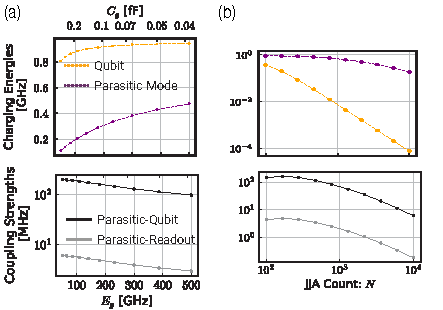
\includegraphics[width=\linewidth]{Supp_Fig/Circuit_comp.pdf}
    \caption{{\bf Dependence of coupling strengths and charging energies on circuit parameters.} (a) parasitic ground capacitance and (b) number of junctions in the array $N$. {\bf (Top row)} The qubit charging energy decides the frequency $\omega_{01}$ and the parasitic charging energy decides the parasitic mode frequency for mode $\mu=2$. {\bf (Bottom row)} give the plots for the coupling strengths of the parasitic mode to readout and qubit, respectively. All plots are obtained under linear JJA approximation.}
    \label{fig:circuit_comp}
\end{figure}

\paragraph{Variation in coupling strength.}\label{coupling} 
We find that achieving low \( g_{\phi\mu} \) requires a low \( C_\textrm{g,j} \) and a high \( N \) (see Fig.~\ref{fig:circuit_comp}). Increasing \( N \) alters the qubit's target inductance, requiring a proportional increase in \( E_{\textrm{J}_\textrm{j}} \) to maintain the inductive energy (\( E_\textrm{L} = E_{\textrm{J}_\textrm{j}}/N \)). However, \( E_{\textrm{J}_\textrm{j}} \) is limited by fabrication constraints, which caps the maximum \( E_\textrm{L} \). This supports the large-\( N \) approximation \( \tilde{E}_{\textrm{c},\mu} \approx 4E_\textrm{g,j}s_\mu^2 \) (Eq.~\ref{eq:parasitic}). Therefore, \( N \) can be optimized to reduce \( g_{\phi\mu} \) while keeping \( E_\textrm{L} \) constant.

However, increasing \( N \) while keeping \( E_\textrm{L} \) and \( E_\textrm{g,j} \) constant also lowers the parasitic charging energy (see Fig.~\ref{fig:circuit_comp}). For large \( N \) and small \( \mu \), 
\begin{align}
 \tilde{E}_{\textrm{c},\mu} \propto 1/N^2,\label{eq:dep2}
\end{align}
which decreases the parasitic mode frequency \( \omega_\mu \) with increasing \( N \). This is generally unfavorable for reducing PMIST, as discussed in the next section. Nonetheless, if the coupling \( g_{\phi\mu} \) is negligible, even low-frequency parasitic modes will not contribute to PMIST effects.
\paragraph{Variation in parasitic charging energy.}\label{par-freq} 
A higher parasitic charging frequency relative to the readout frequency reduces the likelihood of PMIST effects (see Sec.~\ref{sec:expressions}). We find that the parasitic charging energies increase with decreasing \( C_\textrm{g,j} \) and \( N \) (see Fig.~\ref{fig:circuit_comp}). From Eqs.~\ref{eq:dep1}-\ref{eq:dep2}, in the large-\( N \), small-\( \mu \) limit, \( \omega_\mu^\textrm{e} \) is inversely proportional to \( N^2 \) and \( C_\textrm{g,j} \), where \( C_\textrm{g,j} \, [\mathrm{fF}] = 19.4 / E_\textrm{g,j} \, [\mathrm{GHz}] \). Thus, reducing the parasitic ground capacitance \( C_\textrm{g,j} \) increases the charging energy and raises the parasitic mode frequency, which is favorable. 

A smaller \( N \) increases \( g_{\phi\mu} \) but also raises the parasitic mode frequencies, widening the gap between \( \omega_\textrm{d} \) and \( \omega_\mu \), which is beneficial. However, decreasing \( N \) also introduces challenges, such as greater nonlinearity of parasitic modes and stronger coupling strengths. Conversely, a lower \( N \) that reduces \( g_{\phi\mu} \) narrows the frequency gap, which is less favorable. 

These considerations suggest that to minimize PMIST effects, it is crucial to reduce the parasitic ground capacitance in the JJA. Simultaneously, the junction count \( N \) must be carefully optimized to balance parasitic frequencies and qubit-parasitic couplings, while respecting the assumptions of linearity of parasitic modes.
\subsection{Fluxonium qubit Hamiltonian}
We now discuss the parameters related to fluxonium qubit Hamiltonian, through a detailed consideration of its charge matrix elements and the dispersive shifts on the qubit induced by the parasitic modes and readout. The qubit Hamiltonian $H_{\phi}$ (see Eq.~\ref{eq:Hphi}) is diagonalized in the Fock state basis, where we have used the standard bosonic operators
 \begin{equation} \hat x_\phi=x_{\mathrm{ZPF}}(a+a^\dagger)=\hat N_{\phi}/ N_{\phi,\mathrm{ZPF}}
 \end{equation}
 and 
 \begin{equation} \hat p_\phi=-ip_{\mathrm{ZPF}}(a-a^\dagger)=\hat \phi/\phi_{\mathrm{ZPF}}.
 \end{equation}
such that $[\hat x,\hat p]=i$.
\paragraph{Charge matrix elements:}
Here, using the approximations described in App.~\ref{app:alt_circuits}, we calculate the charge matrix elements for the qubit mode. We observe that with increasing final state ($f$), the charge matrix elements with respect to the ground and first two excited states follow a decreasing trend, approximately exponential. This exponential decrease to $10^{-10}$ motivates our truncation of the fluxonium potential up to $30$ levels for the Floquet simulations of Sec.~\ref{sec:MIST}.
\begin{figure}[t]
    \centering
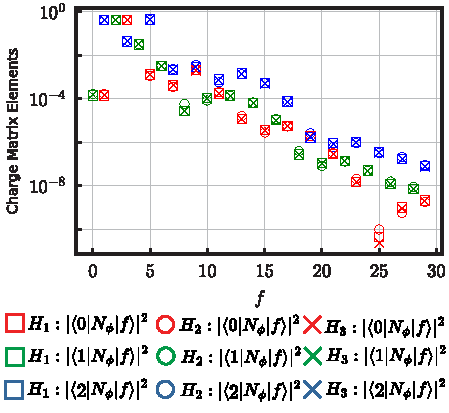
\includegraphics[width=0.45\textwidth]{Supp_Fig/Charge_Matrix.pdf}
    \caption{{\bf Charge matrix 
 elements (squared) for the symmetric circuit.} Note that we use $\langle f|N_\phi|f'\rangle=iN_{\phi,\mathrm{ZPF}}\langle f|(a-a^\dagger)|f'\rangle$ where $N_{\phi,\mathrm{ZPF}}=\frac{1}{\sqrt{2}}\Big(E_{\textrm{J}_\textrm{j}}/8NE_{\textrm{c}}\Big)^{1/4}$. The charge matrix elements between parity conserving states is zero (points not seen in log plot) due to the symmetry of cosine potential at $\varphi_\mathrm{ext}=0.5\Phi_0$, where $\Phi_0$ is the flux quantum.}
    \label{charge-matrix}
\end{figure}


\paragraph{Dispersive Hamiltonian}\label{app:dispersive} 
Next, we extract the qubit parameters quoted in Table~\ref{tab:readout_params}, for example, the dispersive shift of the qubit due to the parasitic modes $\chi_{\phi\mu}$ and the readout mode $\chi_{\phi \textrm{r}}$~\cite{viola2015collective}. These variables were used to generate Fig.~\ref{fig:dephasing} in the main text. For this purpose, we first give the qubit Hamiltonian in the dispersive regime~\cite{viola2015collective},

\allowdisplaybreaks{
\begin{align}
    H/\hbar&=\frac{\omega_\textrm{q}}{2}\sigma_\textrm{z}+\sum_{\mu}(\omega_\mu+k_\mu) a_\mu^\dagger a_\mu
    +\omega_\textrm{r} a_\textrm{r}^\dagger a_\textrm{r}\nonumber\\ &\quad +\chi_{\textrm{r},\phi}\sigma_\textrm{z} a_\textrm{r}^\dagger a_\textrm{r}
    +\sum_{\mu}\chi_{\mu,\phi}\sigma_\textrm{z} a_\mu^\dagger a_\mu\\
   &=\frac{\omega_\textrm{q}}{2}\sigma_\textrm{z}+\Big(\omega_\textrm{r} +\chi_{\phi\textrm{r}}\sigma_\textrm{z}\Big)a_\textrm{r}^\dagger a_\textrm{r}\nonumber\\&+\sum_{\mu}\Big(\omega_\mu+k_\mu+\chi_{\mu\textrm{r}}a_\textrm{r}^\dagger a_\textrm{r}+\chi_{\mu\phi}\sigma_\textrm{z}\Big) a_\mu^\dagger a_\mu\label{eq:dispersive}
\end{align}
where, $\omega_\textrm{q}=\omega_{01}$ is the qubit frequency, $\kappa_\mu$ is the lamb shift on the parasitic mode while all other variables follow the definitions used in Table~\ref{tab:readout_params}. In the main text, we have used the value of the dispersive shift ($\chi_{\phi\mu}$) due to the parasitic mode in Sec.~\ref{sec:dephasing}, computed using the expression from Ref.~\cite{viola2015collective}. For the parameters in Table~\ref{tab:circuit_params}, we plot $\chi_{\phi\mu}$ for all parasitic modes of the symmetric circuit, in Fig.~\ref{fig:dispersive-shift}. We also plot the dispersive shift due to readout $\chi_{\phi \textrm{r}}$ computed using the following expression (derivation not shown here),
\begin{align}  
\chi_{\phi \textrm{r}}&=16g_{\phi\textrm{r}}^2E_{C_\textrm{r}}^2\sqrt{\frac{E_{\textrm{L}_\textrm{r}}}{32E_{C_\textrm{r}}}}\frac{2\epsilon_{01}}{\epsilon_{01}^2-\omega_\textrm{r}^2}|\langle 0|\hat p_\phi|1 \rangle|^2\nonumber\\
   &+16g_{\phi\textrm{r}}^2E_{C_\textrm{r}}^2\sqrt{\frac{E_{\textrm{L}_\textrm{r}}}{32E_{C_\textrm{r}}}}\Bigg[\sum_l|\langle 0|\hat p_\phi|l \rangle|^2\frac{\epsilon_{0l}}{\epsilon_{0l}^2-\omega_\textrm{r}^2}\nonumber\\&\quad-\sum_l|\langle 1|\hat p_\phi|l \rangle|^2\frac{\epsilon_{1l}}{\epsilon_{1l}^2-\omega_\textrm{r}^2}\Bigg]\label{eq:qubit-readout-shift}
\end{align}
\begin{figure}[t]
    \centering
    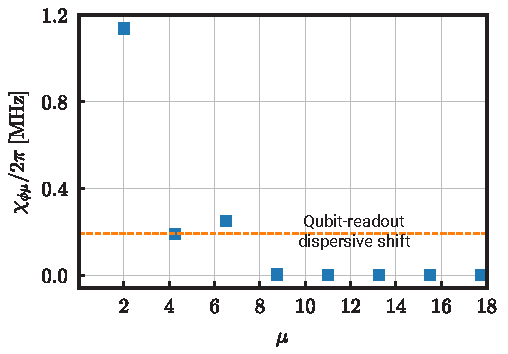
\includegraphics[width=0.45\textwidth]{Supp_Fig/dispersive_shift.pdf}
    \caption{ {\bf The dispersive shift ($\chi_{\phi\mu}$) induced on the qubit due to the parasitic mode $\mu$.} The orange reference line represent the dispersive shift ($\sim $) induced by the readout resonator on the qubit ($\chi_{\mu\textrm{r}}$, see Eq.~\ref{eq:qubit-readout-shift}).}
    \label{fig:dispersive-shift}
\end{figure}

\section{Driven fluxonium circuit}\label{app:MIST}
Here, we discuss the several analysis techniques to study MIST effects used in this work. First, we discuss and justify the Hilbert space truncation, as well as approximations used for Floquet simulations in Sec.~\ref{sec:MIST}. Next, we derive the semi-classical Hamiltonian $H_\textrm{s.c.}$ in Eq.~\ref{eq:drive} and discuss other details related to the Floquet simulations
\subsection{Approximations for numerical modeling}\label{app:numerics}
We use the following three approximations in our work.
\begin{itemize}
    \item \textbf{Restriction to $\mu=2$}. We restrict our analyses to only include the lowest-frequency, even parasitic mode. This mode couples most strongly to the qubit and the readout as evident from Fig.~\ref{fig:coupling-strength}(d). This assumption reduces the Hilbert space size for a feasible study. 

    \item \textbf{Semi-classical drive approximation.}  We treat the readout resonator classically as described in Refs.~\cite{xiao2023diagrammatic,dumas2024unified,cohen2023reminiscence,khezri2023measurement}, eliminating the readout mode states from our numerical simulation. This approximation is again necessary to restrict the Hilbert space size to values feasible for numeric study.
    
    \item \textbf{Linear JJA approximation.} We assume that the parasitic modes are linear, due to the large $E_{\textrm{J}_\textrm{j}}/E_{\textrm{C}_\textrm{j}} \sim 200$ ratio. Nonlinear corrections to our results are beyond the scope of this work. For details on how non-linear corrections affect different circuit energies, we direct the readers to~\cite{viola2015collective}. 
    \item \textbf{Truncation.} We note that the charge matrix elements connecting the fluxonium qubit ground states to excited states decrease roughly exponentially with increasing excited state number (see shown in Fig.~\ref{charge-matrix}). With this observation and our assumptions above, we truncate the Hilbert space dimensions to $20\times 5$. That is, we assume $20$ levels in the fluxonium qubit mode and $5$ levels in the parasitic mode. We justify this truncation in Fig.~\ref{fig:truncation} for all Floquet simulations by giving an analogous plot for Fig.~\ref{fig:Floquet} using a numerical simulation in Hilbert space of $30\times 10$.
    \end{itemize}
    \begin{figure}[t]
        \centering
        \includegraphics[width=0.5\linewidth]{}
        \caption{{\bf Truncation.} Floquet landscape of Fig.~\ref{fig:Floquet} computed using a Hilbert space of $30\times 10$ is shown here. The two plots match in the fluxonium and parasitic levels which get excited at the expected frequencies, as quoted in Table.~\ref{tab:PMIST}.}
        \label{fig:truncation}
    \end{figure}
    Note that for the conclusions drawn in this paper, we are only interested in identifying the existence of PMIST processes, and we do not claim to quantify how many such transitions can be present. Hence, with this truncation we only examine the excitations in $0-20$ levels in the fluxonium subspace in Figs.~\ref{fig:Floquet},~\ref{fig:Flo_low},~\ref{fig:coupling-Floquet}. In this appendix, we show the results for truncating the Hilbert space to $20
    \times 5$ levels in the two modes and $30
    \times 10$, showing the convergence of the MIST results. Importantly, both simulations show no higher than excitation of $\bar n_\mu=2$ in parasitic mode.

\subsection{Semi-classical approximation}\label{app:semi-classical}
In this Appendix, we derive the semiclassical Hamiltonian $H_\textrm{s.c.}$ (see Eq.~\ref{eq:drive_Ham}) used for the Floquet simulations. The fully quantum Hamiltonian is given by 
\begin{align}
    H_\textrm{drive}=\hat H \textrm{ (see Eq.~\ref{Hamiltonian_total}) }-i\epsilon_\textrm{d}(\hat a_\textrm{r}-\hat a_\textrm{r}^\dagger)\sin{\omega_\textrm{d} t}
\end{align}
where $\omega_\textrm{d}$ is the drive frequency and $\epsilon_\textrm{d}\in \mathbb{R}$ is the drive strength. For the semi-classical approximation, we first use the rotating frame transformation $UH_\textrm{drive}U^\dagger-i\dot{U}U^\dagger$ under the unitary $U=e^{-i\hat H_\textrm{r}t}=e^{-i\omega_\textrm{r} \hat a_\textrm{r}^\dagger \hat a_\textrm{r}t}$. This transformation imposes $a_\textrm{r}\rightarrow a_\textrm{r}e^{-i\omega_\textrm{r}t}=\hat{\tilde{a}}$. Now, in the interaction picture we have $U\hat H_\textrm{drive}U^\dagger+i\dot{U}U^\dagger$ (ignoring terms which oscillate at a rate faster than $\omega_\textrm{d}=\omega_\textrm{r}$),
\begin{align}
   =&\hat H_\phi+\sum_{\mu\in 2\mathbb{Z}}\hat H_\mu+\frac{g_{\phi\mu}\hat N_\phi\hat N_\mu}{N_{\phi,\textrm{ZPF}}N_{\mu,\textrm{ZPF}}}+\frac{\epsilon_\textrm{d}}{2}(\hat a_\textrm{r}+\hat a_\textrm{r}^\dagger)\nonumber\\ 
   &-i\frac{g_{\phi\textrm{r}}\hat N_\phi}{N_{\phi,\textrm{ZPF}}}(\hat {\tilde{a}}_\textrm{r}-\hat {\tilde{a}}_\textrm{r}^\dagger)-i\frac{g_{\mu\textrm{r}}\hat N_\mu}{N_{\mu,\textrm{ZPF}}}(\hat {\tilde{a}}_\textrm{r}-\hat {\tilde{a}}_\textrm{r}^\dagger)
\end{align}
Let us call the Hamiltonian at this stage, $H_\textrm{U}$. Now we go to the displaced frame $a_\textrm{r}\rightarrow a_\textrm{r}+\alpha$ via transformation under the unitary $U_\alpha=e^{-i\alpha(\hat a_\textrm{r}+\hat a_\textrm{r}^\dagger)}$ such that in the interaction picture we have $ U_\alpha\hat H_\textrm{U}U_\alpha^\dagger+i\dot{U}_\alpha U_\alpha^\dagger$ 
\begin{align}
   =&\hat H_\phi+\sum_{\mu\in 2\mathbb{Z}}\hat H_\mu+\frac{g_{\phi\mu}\hat N_\phi\hat N_\mu}{N_{\phi,\textrm{ZPF}}N_{\mu,\textrm{ZPF}}}\label{bare}\\ 
   &-i\frac{g_{\phi\textrm{r}}\hat N_\phi}{N_{\phi,\textrm{ZPF}}}(\hat {\tilde{a}}_\textrm{r}-\hat {\tilde{a}}_\textrm{r}^\dagger)-i\frac{g_{\mu\textrm{r}}\hat N_\mu}{N_{\mu,\textrm{ZPF}}}(\hat {\tilde{a}}_\textrm{r}-\hat {\tilde{a}}_\textrm{r}^\dagger)\label{quantum}\\
   &-i\frac{g_{\phi\textrm{r}}\hat N_\phi}{N_{\phi,\textrm{ZPF}}}(\alpha e^{-i\omega_\textrm{r} t}-\alpha^* e^{i\omega_\textrm{r} t})\\&-i\frac{g_{\mu\textrm{r}}\hat N_\mu}{N_{\mu,\textrm{ZPF}}}(\alpha e^{-i\omega_\textrm{r} t}-\alpha^* e^{i\omega_\textrm{r} t})\label{classical}\\
   &-\frac{\epsilon_\textrm{d}}{2}(\hat a_\textrm{r}+\hat a_\textrm{r}^\dagger)+\dot{\alpha}(\hat a_\textrm{r}+\hat a_\textrm{r}^\dagger)\label{drive}
\end{align}
We choose $\dot{\alpha}=\frac{\epsilon_\textrm{d}}{2}\implies\alpha(t)\in\mathbb{R}$ to remove the terms in Eq.~\ref{drive}, such that the Eq.~\ref{classical} take the form,
\begin{align}
    -\Big[\frac{g_{\phi\textrm{r}}\hat N_\phi}{N_{\phi,\textrm{ZPF}}}+\frac{g_{\mu\textrm{r}}\hat N_\mu}{N_{\mu,\textrm{ZPF}}}\Big](2\alpha\cos{\omega_\textrm{d} t})\label{semi-classical}
\end{align}
Now, we go back to the lab frame and ignore the terms associated with the quantum operators $\hat{\tilde{a}}_\textrm{r}$ in Eqs.~\ref{quantum} while we replace $\alpha$ with the mean value $\sqrt{\bar n_\textrm{r}}$ in the term~\ref{semi-classical} to get the final semi-classical form $H_\textrm{s.c.}$~\cite{cohen2023reminiscence}.

\subsection{Floquet simulations}
\paragraph{Stark shift:}\label{app:stark-shift}
To observe a state transition, the primary requirements are high charge matrix elements and low energy difference. The eigenenergies of the states in question are changed with an increase in the number of readout photons or, in this case, the drive strength. In this section, we compute the Stark-shifted eigenenergies which facilitate the prediction of an avoided crossing using a first-order perturbative approach, given $\bar n_\textrm{r}, \omega_\textrm{r}$ and the charge matrix elements.  Let $\ket{i}$ be a state in the eigenspace of $H_{\textrm{int}}=H_\phi+H_{\mu=2}+g_{\phi\mu}\hat N_\phi\hat N_\mu$. Following derivations in App.~\ref{app:Hamiltonian}, the Stark-shift in the energy of state $\ket{i}$ at an average number of readout photons $\bar n_\textrm{r}$ is given by
\begin{align}
    \chi_i(\bar n_\textrm{r})=2\bar n_\textrm{r}\sum_{f}\omega_{if}\Big[\frac{g_{\phi \textrm{r}}|\braket{i|\hat N_\phi|f}|^2}{\omega_\textrm{d}^2-\omega_{if}^2}+\frac{g_{\mu \textrm{r}}|\braket{i|\hat N_\mu|f}|^2}{\omega_\textrm{d}^2-\omega_{if}^2}\Big]\label{eq:stark}
\end{align}
 Here $\omega_{if}=E_f-E_i$ denote the energy difference in the eigen-energies of the state $\ket{i}$. The impact due to the second term is much smaller than the first term, and hence $g_{\phi \textrm{r}}$ primarily governs this Stark shift.
 \begin{figure}
     \centering
     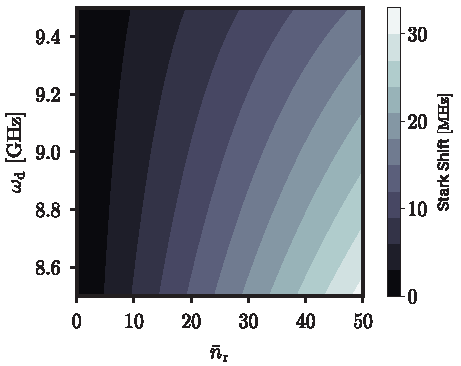
\includegraphics[width=\linewidth]{Supp_Fig/Stark-shift.pdf}
     \caption{\textbf{Stark shift in the ground state of fluxonium due to readout.} Values are computed using Eq.~\ref{eq:stark} for energy level $i=\ket{\tilde{0},\tilde{0}}$. We have verified that Stark shift on the excited energy levels $\ket{\tilde{1},\tilde{0}}$ and $\ket{\tilde{2},\tilde{0}}$ are also upper bounded by $50$ MHz for the ranges of $\omega_\textrm{d}$ and $ \bar n_\textrm{r}$ considered in this plot.}
     \label{fig:stark-shift}
 \end{figure}

\paragraph{Population exchange and quasienergies:}\label{app:Floquet-trans}
Below we plot the population exchange and quasi-energy probabilities for all transitions captured in Fig.~\ref{fig:Floquet} and Table~\ref{tab:PMIST} for states $\ket{\tilde{0},\tilde{0}}$ (see Fig.~\ref{fig:Trans0}), $\ket{\tilde{1},\tilde{0}}$ (see Fig.~\ref{fig:Trans1}) and $\ket{\tilde{2},\tilde{0}}$ (see Fig.~\ref{fig:Trans2}). We will comment on some special types of transitions explicitly here.

\begin{itemize}
    \item Transition $(2)$ has two crossings, one that takes place at $\bar n_\textrm{r}=14$ and another at $\bar n_\textrm{r}=48$. The states $\ket{\tilde{4},\tilde{2}}$ and $\ket{\tilde{14},\tilde{2}}$ hybridize first and then the resulting state hybridizes with the computational state $\ket{\tilde{0},\tilde{0}}$.
    \item Transitions $(3,4)$ show a branch bunching scenario, as quoted in Ref.~\cite{dumas2024unified} for the case of positive detuning. However, in this case we note that both branch bunching and crossings were observed in the negative detuning case. Such branch bunching occurs when the drive frequency $(\omega_\textrm{d})$ is equal to the transition frequency of two states $i,j (\omega_{ij})$. In the presence of parasitic mode, there are multiple states ($\ket{\tilde{i},\tilde{\mu
    }}$ and $\ket{\tilde{j},\tilde{\mu}}$ for various $\mu$) such that $\omega_\textrm{d}=\omega_{ij}$ is the resonant frequency for the observation of bunching between the two states.
    \item In transitions $(9,11,12)$ the states do not return to the same population as the initial states. This is the case because we are plotting the bare fluxonium and parasitic mode operators $\braket{\bar n_\phi},\braket{\bar n_\mu}$. We make this choice to show the impact of PMIST effects on the bare fluxonium population since the parasitic modes have been ignored in most previous fluxonium analyses.
    \item Finally, in transition $(14)$ we again see two crossings. In the absence of qubit-parasitic coupling $g_{\phi\mu}$ this transition is only carried out between  $\ket{\tilde{17},\tilde{0}}$ and $\ket{\tilde{2},\tilde{0}}$. However, in the presence of parasitic modes $\ket{\tilde{17},\tilde{0}}$ hybridizes with $\ket{\tilde{5},\tilde{1}}$ which then has a branch crossing with $\ket{\tilde{2},\tilde{0}}$. Thus, in this case we see that ignoring parasitic modes can lead to wrong state predictions which could affect the qubit reset post measurement.
\end{itemize}

\paragraph{Landau-Zener probabilities:}\label{app:LZ}
We compute the Landau-Zener probabilities in Sec.~\ref{sec:LZ} numerically using the quasienergies from the Floquet simulations, and analytically, using the Stark-shifted eigen-energies. In this case, we use a time-dependent readout photon number, where $\bar n_\textrm{r}$ varies as $\bar n_\textrm{r}=50(1-e^{-\kappa t/2})^2$, to emulate change in readout photons from dissipation~\cite{dumas2024unifie,khezri2023measurement}. The numerical calculations use the probability for Landau-Zener transitions given in~\cite{ikeda2022floquet}, for an avoided crossing observed between states $\ket{i},\ket{f}$ of
\begin{align}
    P_\textrm{LZ}&=\exp{\Big[-\frac{\pi \Delta_\textrm{ac}^2}{2v}\Big]},\\
    \text{where } v&=\sqrt{2\Delta_\textrm{ac}\Big|\frac{d^2\epsilon_f}{d\sqrt{\bar{n}_\textrm{r}(t)}^2}\Big|_{t_\textrm{ac}}}\frac{d\sqrt{\bar{n}_\textrm{r}(t)}}{dt}|_{t_\textrm{ac}}\Big .
\end{align}
Here, the variable $\epsilon_f$ is the numerically-computed quasi-energy obtained from Floquet simulations, while $\Delta_\textrm{ac}$ refers to their quasi-energy difference at avoided crossing. 

\section{Alternative circuit parameters}\label{app:alt_circuit1}
Here, we give the circuit parameters (Table~\ref{tab:circuit_params_Will}), coupling strengths (Fig.~\ref{fig:coupling-strength-Will}), charge matrix elements (Fig.~\ref{fig:charge-matrix-Will}) and state transition quasienergies shown in Figs.~\ref{fig:Floquet1} and Fig.~\ref{fig:011_Will}. 
%The truncation for these simulations uses the same justification and assumptions as App.~\ref{app:numerics}. 
\begin{table}[htb]
\centering
\begin{tabular}{|c|c|c|c|c|c|c|c|c|c|}
    \hline
     $N$ & $\varphi_{\textrm{ext}}$ & $E_{\textrm{J}_\textrm{p}}$ & $E_{\textrm{C}_\textrm{p}}$ & $E_{\textrm{C}}$ & $E_{\textrm{C}_\textrm{j}}$ & $E_{\textrm{J}_\textrm{j}}$ & $E_{C_\textrm{g,j}}$ & $E_{C_\textrm{g,p}}$ & $E_{\textrm{c}}$ \\
    \hline
    $102$ & $0.5\Phi_0$ & $6.20$ & $1.24$ & $4.28$ & $0.74$ & $81.6$ & $194$ & $1.94$ & $19.40$ \\
    \hline
\end{tabular}
\caption{\textbf{Circuit parameters for Fig.~\ref{fig:Floquet1}(a) inspired by Ref.~\cite{ding_high-fidelity_2023}.} All energies are given in GHz. Here $\Phi_0=h/2e$ denotes the magnetic flux quantum. The capacitive energies $E_{\textrm{C}}=\frac{19.4}{{C}(fF)} \ \mathrm{GHz}$ are computed from the corresponding capacitances $C'$.}
\label{tab:circuit_params_Will}
\end{table}

The coupling strengths in this circuit are similar to those evaluated for our original circuit parameters, in Fig.~\ref{fig:coupling-strength}. We find in Fig.~\ref{fig:charge-matrix-Will} that the charge matrix elements of the second circuit analyzed in Sec.~\ref{Will_circuit} has a faster decrease with increasing excited state levels. This could be indicative of the fact that such a circuit will see lower MIST effects as observed in Fig.~\ref{fig:Floquet1}(c). Finally, we plot the PMIST effect observed in the Floquet simulations for this alternative circuit in Fig.~\ref{fig:011_Will}. We perform a branch analysis of the initial state $\ket{\tilde{0}, \tilde{0}}$ and observe a transition to $\ket{\tilde{4},\tilde{1}}$, as described in the main text. 
\begin{figure*}
    \centering
    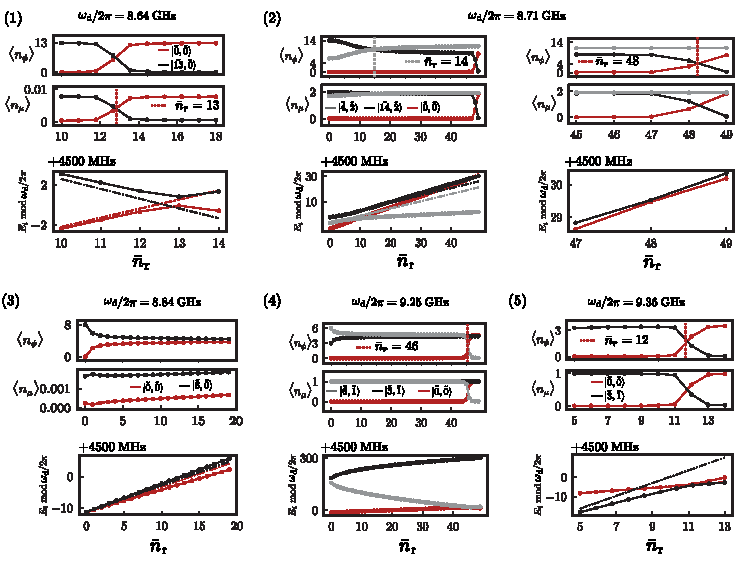
\includegraphics[width=1.0\textwidth]{Supp_Fig/Trans0.pdf}
    \caption{\textbf{MIST processes from Table~\ref{tab:PMIST} involving the $\ket{\tilde{0},\tilde{0}}$ state.} The figure numbering indicates the row index in Table~\ref{tab:PMIST}. (Top row) Fluxonium subspace $\braket{n_\phi}$. (Middle) Parasitic mode subspace $\braket{n_\mu}$ (Bottom) Stark-shifted eigen-energies (dashed) and quasi-energies (solid) from Floquet simulations, corresponding to the initial state $i$ as per the legend. The y-axis for this plot is in MHz. Floquet results are extracted from numerical data used for Fig.~\ref{fig:Floquet}. Note that MIST in figure $(2)$ is split into two figures in order to capture the two consecutive transitions involved.}
    \label{fig:Trans0}
\end{figure*}
\begin{figure*}
    \centering
    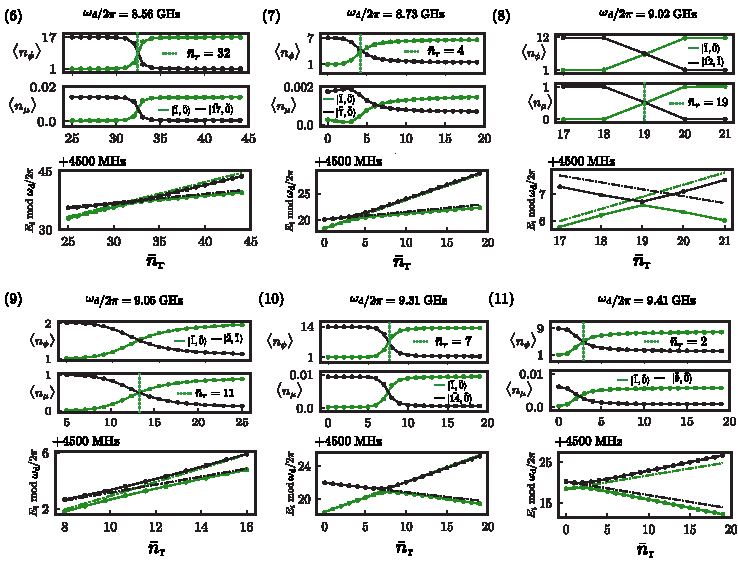
\includegraphics[width=1.0\textwidth]{Supp_Fig/Trans1.pdf}
    \caption{\textbf{MIST processes from Table~\ref{tab:PMIST} involving the $\ket{\tilde{1},\tilde{0}}$ state.} The figure numbering indicates the row index in Table~\ref{tab:PMIST}. (Top row) Fluxonium subspace $\braket{n_\phi}$. (Middle) Parasitic mode subspace $\braket{n_\mu}$ (Bottom) Stark-shifted eigen-energies (dashed) and quasi-energies (solid) from Floquet simulations, corresponding to the initial state $i$ as per the legend. The y-axis for this plot is in MHz. Floquet results are extracted from numerical data used for Fig.~\ref{fig:Floquet}.}
    \label{fig:Trans1}
\end{figure*}
\begin{figure*}
    \centering
    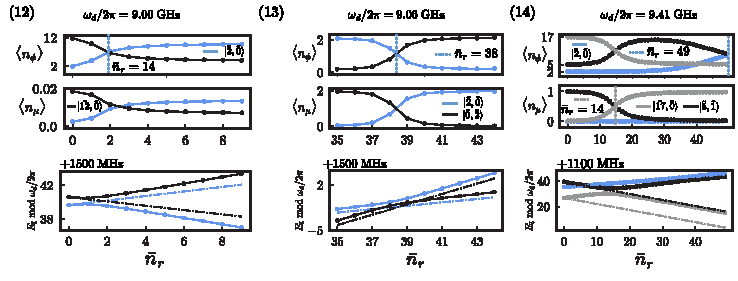
\includegraphics[width=1.0\textwidth]{Supp_Fig/Trans2.pdf}
    \caption{\textbf{MIST processes from Table~\ref{tab:PMIST} involving the $\ket{\tilde{2},\tilde{0}}$ state.} The figure numbering indicates the row index in Table~\ref{tab:PMIST}. (Top row) Fluxonium subspace $\braket{n_\phi}$. (Middle) Parasitic mode subspace $\braket{n_\mu}$ (Bottom) Stark-shifted eigen-energies (dashed) and quasi-energies (solid) from Floquet simulations, corresponding to the initial state $i$ as per the legend. The y-axis for this plot is in MHz. Floquet results are extracted from numerical data used for Fig.~\ref{fig:Floquet}.}
    \label{fig:Trans2}
\end{figure*}
\begin{figure}[htb]
    \centering
    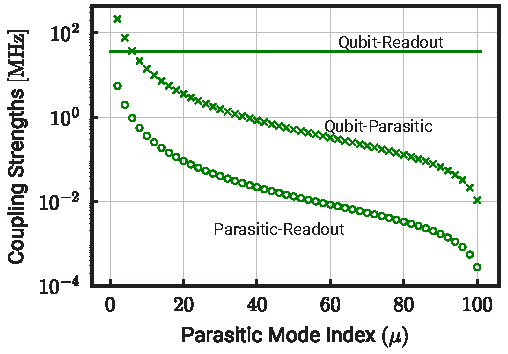
\includegraphics[width=\linewidth]{Supp_Fig/Coupling-Will.pdf}
    \caption{{\bf Absolute values of the coupling strengths for parameters in Table.~\ref{tab:circuit_params_Will}.} $g_{\phi \textrm{r}}/2\pi$ (qubit-readout), $g_{\phi\mu}/2\pi$ (qubit-parasitic), $g_{\mu \textrm{r}}/2\pi$ (parasitic-readout), for various circuits. Coupling to odd parasitic modes is zero due to the symmetries of the circuit~\cite{viola2015collective}. The parasitic modes $\mu\in\{2,4,6\}$ couple to the qubit more or as strongly as the readout.}
    \label{fig:coupling-strength-Will}
\end{figure}
\begin{figure}[htb]
    \centering
    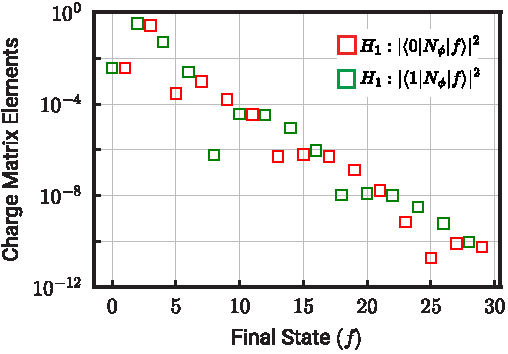
\includegraphics[width=\linewidth]{Supp_Fig/Charge-matrix-Will.pdf}
    \caption{{\bf Charge matrix 
 elements (squared) for parameters in Table.~\ref{tab:circuit_params_Will}.} Note that in the equations below we substitute $\langle i|N_\phi|f\rangle=iN_{\phi,\mathrm{ZPF}}\langle i|(a-a^\dagger)|f\rangle$ where $N_{\phi,\mathrm{ZPF}}=\frac{1}{\sqrt{2}}\Big(E_{\textrm{J}_\textrm{j}}/8NE_{\textrm{C}}\Big)^{1/4}$. The charge matrix elements between odd-odd or even-even is zero (points not seen in log plot) due to the symmetry of cosine potential at $\varphi_\mathrm{ext}=0.5\Phi_0$, where $\Phi_0$ is the flux quantum.}
    \label{fig:charge-matrix-Will}
\end{figure}

\begin{figure}[htb]
    \centering
    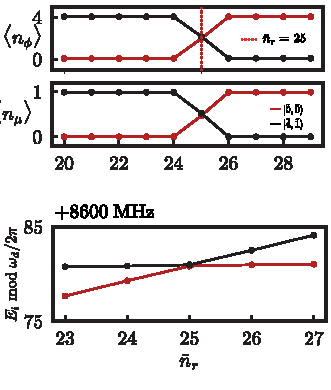
\includegraphics[width=\linewidth]{Supp_Fig/Floquet_Will_landscape.pdf}
    \caption{{\bf Examples of PMIST using transitions for the alternative circuit in Fig.~\ref{fig:Floquet1}(c) of Sec.~\ref{Will_circuit}.} involving the states $\ket{\tilde{0},\tilde{0}}\leftrightarrow\ket{\tilde{4},\tilde{1}}$, with maximum overlap to the un-hybridized state $\ket{k}_\phi\otimes\ket{n}_{\mu=2}$. \textbf{Top row:} Qubit mode average occupation $\braket{n_\phi}$. \textbf{Middle row:} Parasitic mode average occupation $\braket{n_\mu}$. \textbf{Bottom row:} Quasi-energies (solid) from Floquet simulations showing avoided crossings. Plots are extracted from numerical data used in Fig.~\ref{fig:Floquet}. The data points are connected by lines for visual aid.}
    \label{fig:011_Will}
\end{figure}

\clearpage
\bibliography{refs.bib} 
\end{document}

